
%%%%%%%%%%%%%%%%%%%%%%%%%%%%%%%%%%%%%%%%%%%%%%%%%%%%%%%%%%%%%%%%%%%%
%% I, the copyright holder of this work, release this work into the
%% public domain. This applies worldwide. In some countries this may
%% not be legally possible; if so: I grant anyone the right to use
%% this work for any purpose, without any conditions, unless such
%% conditions are required by law.
%%%%%%%%%%%%%%%%%%%%%%%%%%%%%%%%%%%%%%%%%%%%%%%%%%%%%%%%%%%%%%%%%%%%

\documentclass[compress]{beamer}
\usetheme[faculty=phil, navigation, microtype]{fibeamer}
%\usetheme[logo=resources/NOKIA]{fibeamer}
\useoutertheme{miniframes}
\setbeamercolor{section in head/foot}{fg=white, bg=fibeamer@blue}
\usepackage[french]{babel}
\usepackage[utf8]{inputenc}
\usepackage[T1]{fontenc}
\title{seL4: Formal verification of an OS kernel} %% that will be typeset on the
\author{Clément Tamines \& Florent Delgrange}
\vspace{0.5cm}
\subtitle{\normalsize UMONS \\ Faculty of Science \\ Mab2 Computer Science}
\date{\today}
%% These additional packages are used within the document:
\usepackage{ragged2e}  % `\justifying` text
\usepackage{cancel}
\usepackage{bbold}
\usepackage{booktabs}  % Tables
\usepackage{slashed}
\usepackage{centernot}
\usepackage{tabularx}
\usepackage{tikz}      % Diagrams
\usetikzlibrary{calc, shapes, backgrounds}
\usepackage{arevmath}
\usepackage{amsmath, amssymb}
\usepackage{url}       % `\url`s
\usepackage{changepage}
\usepackage{cprotect}
\usepackage{caption}
\usepackage{graphicx}
\usepackage{minted}
\usepackage{biblatex}
\usepackage{mathtools}
\usepackage{multicol}
\usepackage{bbold}
\usepackage[normalem]{ulem}
\usepackage{verbatim}
\usepackage{minted}
%\usepackage{pstricks,pst-node}
%\usepackage{fancyvrb}
%\usepackage{listings}


\definecolor{DarkOrange}{HTML}{FF8C00}
\newtheorem{theoreme}{Theorem}
\newtheorem{lemme}{Lemma}

\title{AI: Deep Learning for\\\vspace{-.05\linewidth} Computer Vision $\quad  \quad \quad \quad \quad$
\includegraphics[width=0.2\linewidth]{resources/eye}\\
{\normalsize A Data Science Approach}} %% that will be typeset on the
%\subtitle{Presentation Subtitle} %% title page.

\bibliography{bib}
\begin{document}
  \begin{frame}[plain]
    \maketitle
  \end{frame}

  \AtBeginSection[]
    {
      %  \begin{frame}<beamer>
      %  \frametitle{Plan}
      %  \tableofcontents[currentsection]
      %  \end{frame}
      \begin{frame}{\contentsname}
      %\vspace{-0.05\linewidth}
      \tableofcontents[currentsection]
      \end{frame}
    }

\begin{frame}{Table des matières}
  \tableofcontents
\end{frame}

\section{Introduction}
\subsection{Machine learning}
\begin{frame}{Machine learning}
  \begin{itemize}
    \item Capacité d'\textbf{\color{fibeamer@orange}apprendre} à l'aide d'une \textbf{\color{fibeamer@orange}base de données}
    \begin{itemize}
      \item[$\rightarrow$] \textbf{\color{fibeamer@orange}Nettoyage des données}: données invalides, non-complètes, non-uniformes, etc.
      \item[$\rightarrow$] \textbf{\color{fibeamer@orange}Préparation des données}: \textbf{uniformiser} l'encodage des \textit{instances} du jeu de données et ses \textit{attributs}
      \item[$\rightarrow$] \textbf{\color{fibeamer@orange} Big Data}
    \end{itemize}
    \item \textbf{\color{fibeamer@orange}Entraînement} de \textbf{\color{fibeamer@orange}modèles} grâce à ces données
    \item Modèles \textbf{\color{fibeamer@orange}prédictifs}
    \begin{itemize}
      \item[$\rightarrow$] classification
        $\quad$ exemple : homme/femme ?
      \item[$\rightarrow$] régression $ \quad \quad$
        exemple : âge ?
    \end{itemize}
  \end{itemize}
\end{frame}

\begin{frame}{Entraînement}{Exemple : Iris database}
  %\vspace{-.05\linewidth}
  \begin{figure}
    \centering
    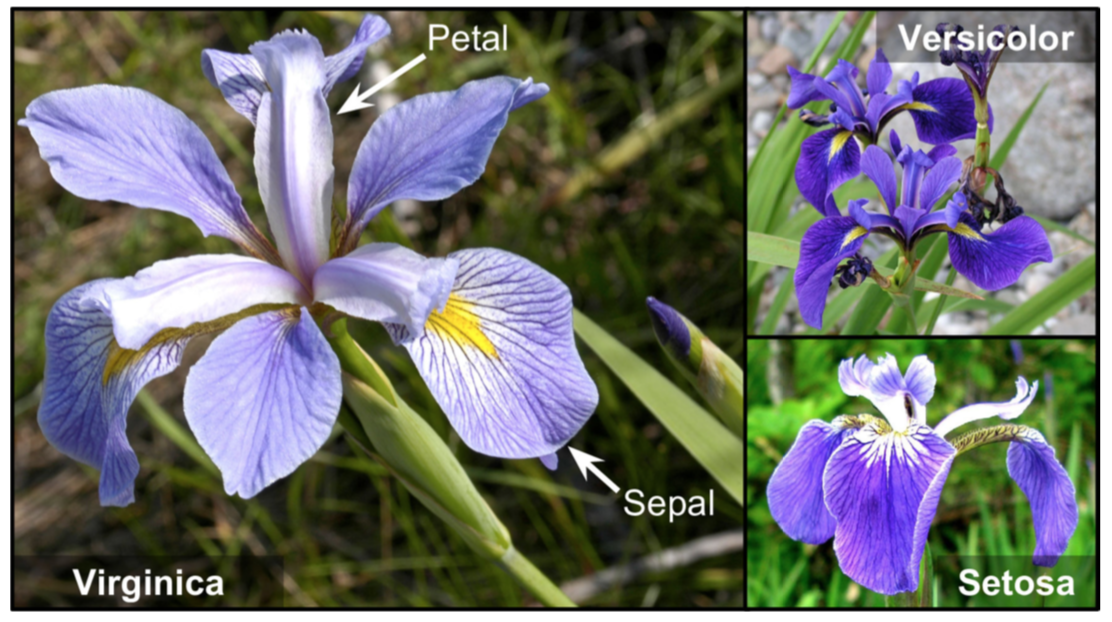
\includegraphics[width=0.7\linewidth]{resources/iris}
  \end{figure}
  \vspace{-.05\linewidth}
  \begin{itemize}
    \item \textbf{\color{fibeamer@orange}Attributs}: longueur des sépales et des pétales, largeur des sépales et des pétales
    \item \textbf{\color{fibeamer@orange}Labels}: Iris Virginica, Iris Versicolors, Iris Setosa
    %\item \textit{\color{fibeamer@blue}Exemple $\rightarrow$ instance $i$}:
    %$x^{(i)}=(5.1, 3.5, 1.4, 0.2)$, $y^{(i)} = (I. \, Setosa)$
  \end{itemize}
\end{frame}

\begin{frame}{Entraînement} \footnotesize
  \begin{figure}
  \centering
  \alt<2>{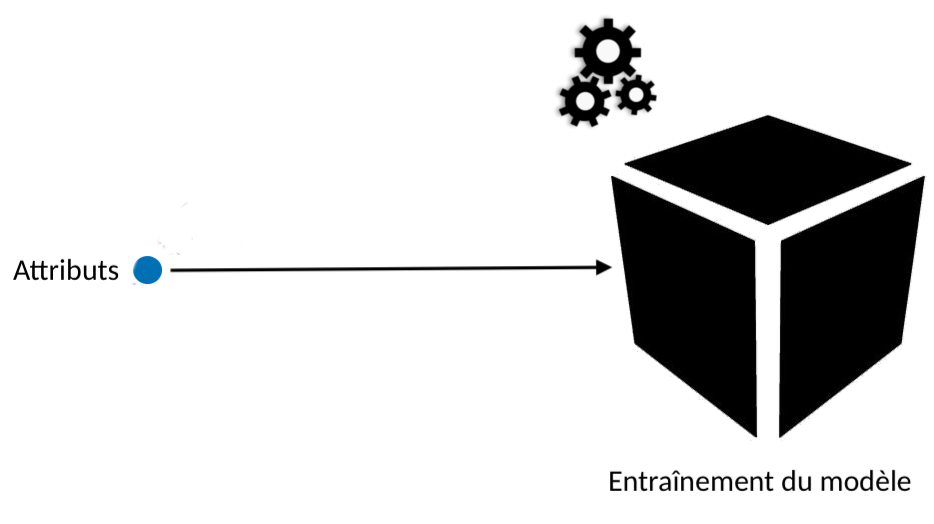
\includegraphics[width=0.7\linewidth]{resources/resume1}}{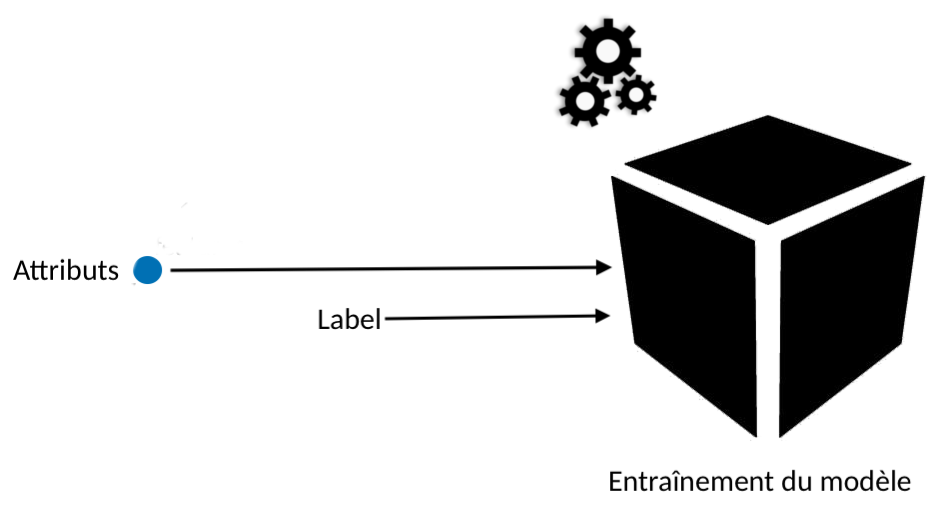
\includegraphics[width=0.7\linewidth]{resources/resume3}}
  \end{figure}
  \begin{itemize}
    \item<1-> \textbf{\color{fibeamer@orange}Entraînement supervisé} : le modèle s'entraîne sur base des attributs et des \textit{\color{fibeamer@orange}labels} des instances {\color{fibeamer@blue}+} apprend à reconnaître les labels des instances
    \item<2-> \textbf{\color{fibeamer@orange}Entraînement non-supervisé} : le modèle apprend à séparer les données et à les classer uniquement sur base des attributs (\textbf{\color{fibeamer@orange}clustering})
  \end{itemize}
\end{frame}

\begin{frame}{Prédictions}
  \begin{figure}
  \centering
  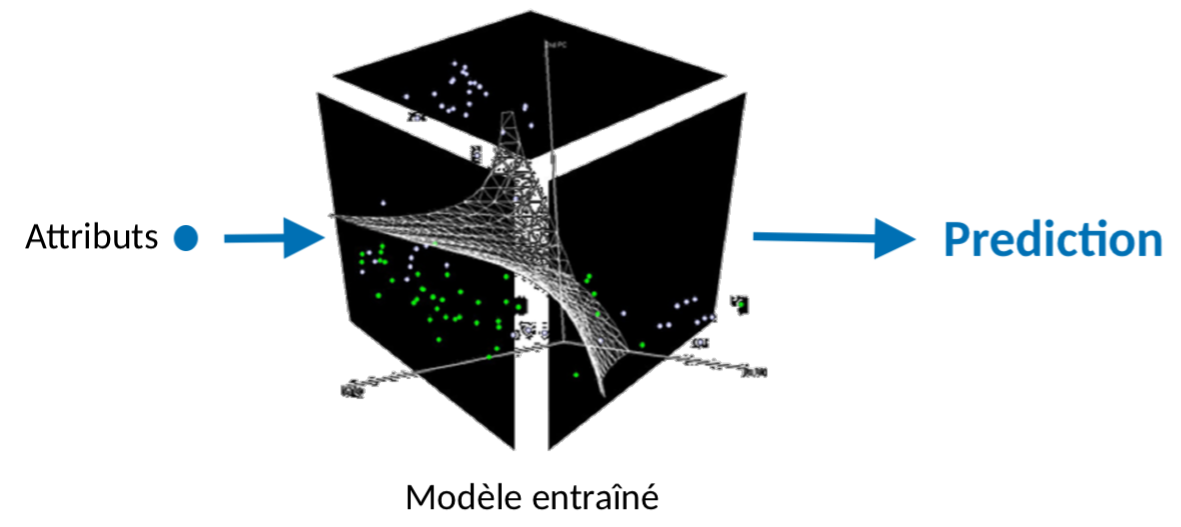
\includegraphics[width=0.7\linewidth]{resources/resume2}
  \end{figure}
  \vspace{-.05\linewidth}
  \begin{itemize}
    \item \textbf{\color{fibeamer@orange}Exemple} : selon les longueurs/largeurs des sépales et pétales, prédire l'espèce d'Iris (classifieur)
    \item \textbf{\color{fibeamer@orange}Remarque} : Un régresseur peut être vu comme une fonction
    \[ f: \mathbb{R}^n \, \rightarrow \, \mathbb{R}, \; x_1, x_2, \dots x_n \mapsto f(x_1, x_2, \dots, x_n)\]
    où $(x_i)_{1\leq i \leq n}$ est un vecteur de $n$ attributs
  \end{itemize}
\end{frame}

\begin{frame}{Types de modèles}
  \begin{adjustwidth}{-2.5em}{-2.5em}
  \begin{columns}
    \begin{column}{0.33\textwidth}
      \centering
      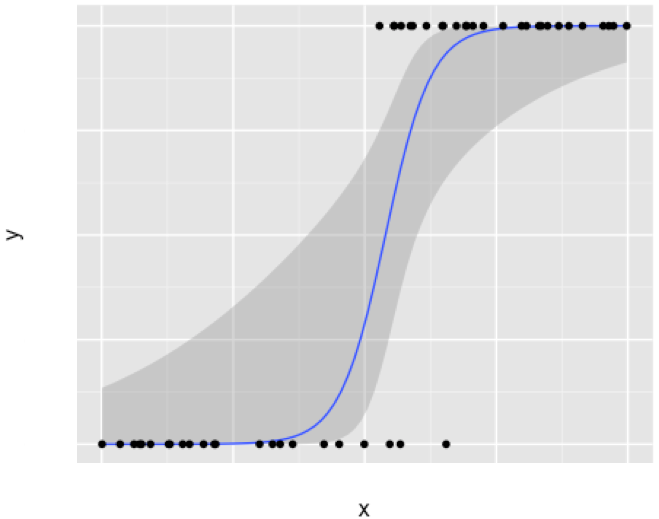
\includegraphics[width=\textwidth]{resources/logreg}
      \\{\footnotesize Régression logistique}
    \end{column}
    \begin{column}{0.33\textwidth}
      \centering
      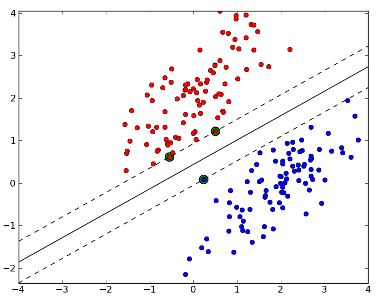
\includegraphics[width=0.85\textwidth]{resources/lsvm}\\
      {\footnotesize Machine à vecteurs de support}
    \end{column}
    \begin{column}{0.33\textwidth}
      \centering
      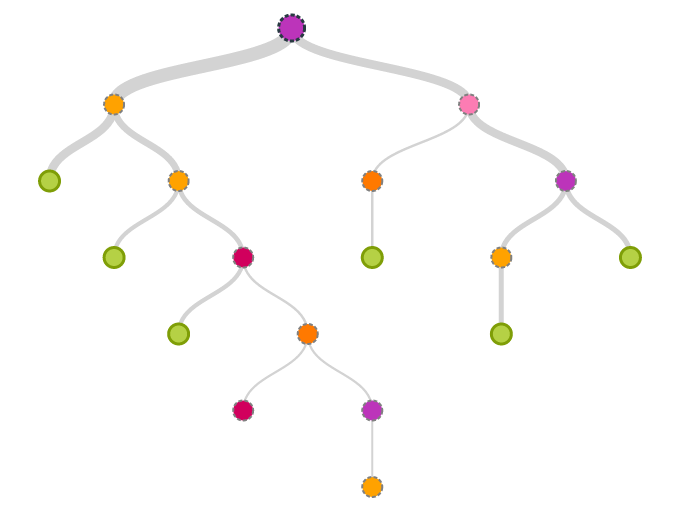
\includegraphics[width=\textwidth]{resources/CART}\\
      {\footnotesize Arbre de décisions (CART)}
    \end{column}
  \end{columns}
  \vspace{0.5cm}
  \begin{columns}
   \begin{column}{0.33\textwidth}
     \centering
     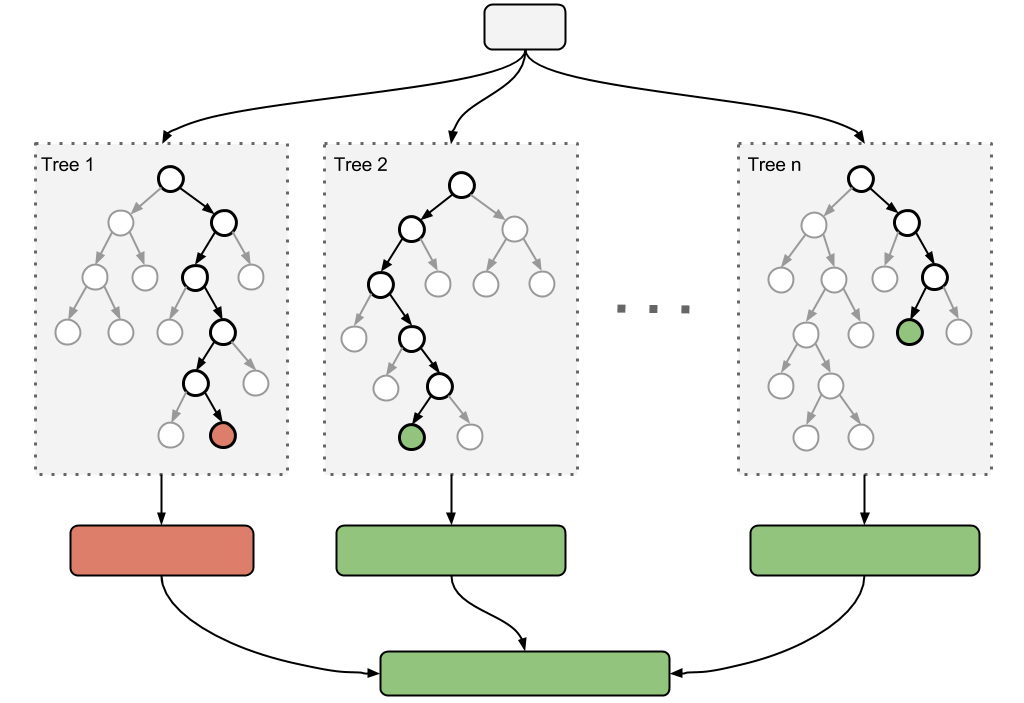
\includegraphics[width=0.9\textwidth]{resources/random_forest}\\
     {\footnotesize Forêt aléatoire}
   \end{column}
   \begin{column}{0.33\textwidth}
     \centering
     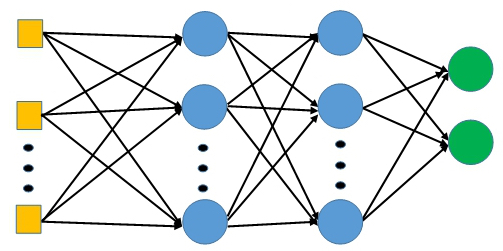
\includegraphics[width=\textwidth]{resources/MLP}\\
     {\footnotesize Perceptron à couches multiples (RNN)}
   \end{column}
   \begin{column}{0.33\textwidth}
     \centering
     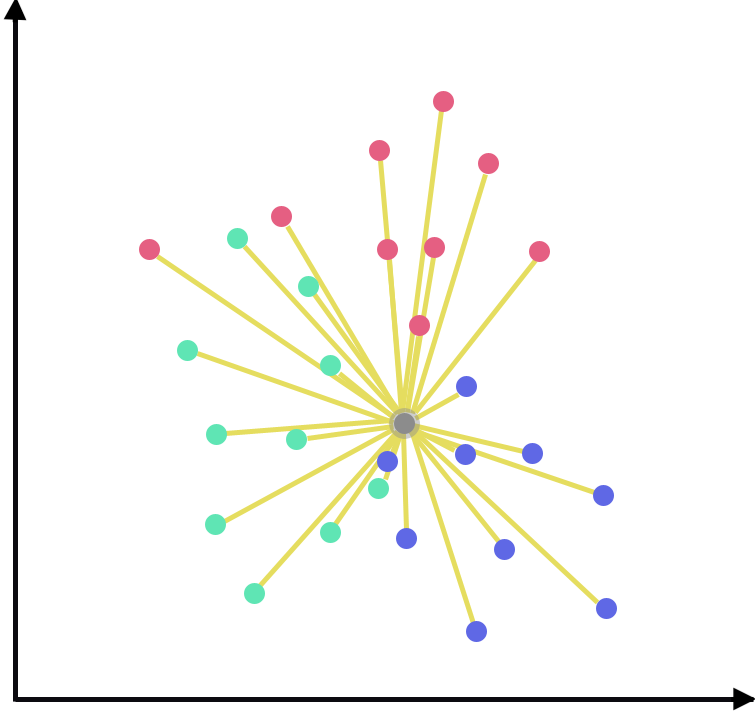
\includegraphics[width=0.65\textwidth]{resources/knn}\\
     {\footnotesize Autres (kNN, Naive Bayes, etc.)}
   \end{column}
  \end{columns}
  \end{adjustwidth}
\end{frame}

\subsection{Signal}
\begin{frame}{Traitement du signal pour le machine learning}
  \begin{itemize}
    \item Une image numérique est un signal discret en 2 dimensions
    \begin{itemize}
      \item[$\rightarrow$] 3 matrices de valeurs de 0 à 255 (RGB)
    \end{itemize}
    \begin{center}
      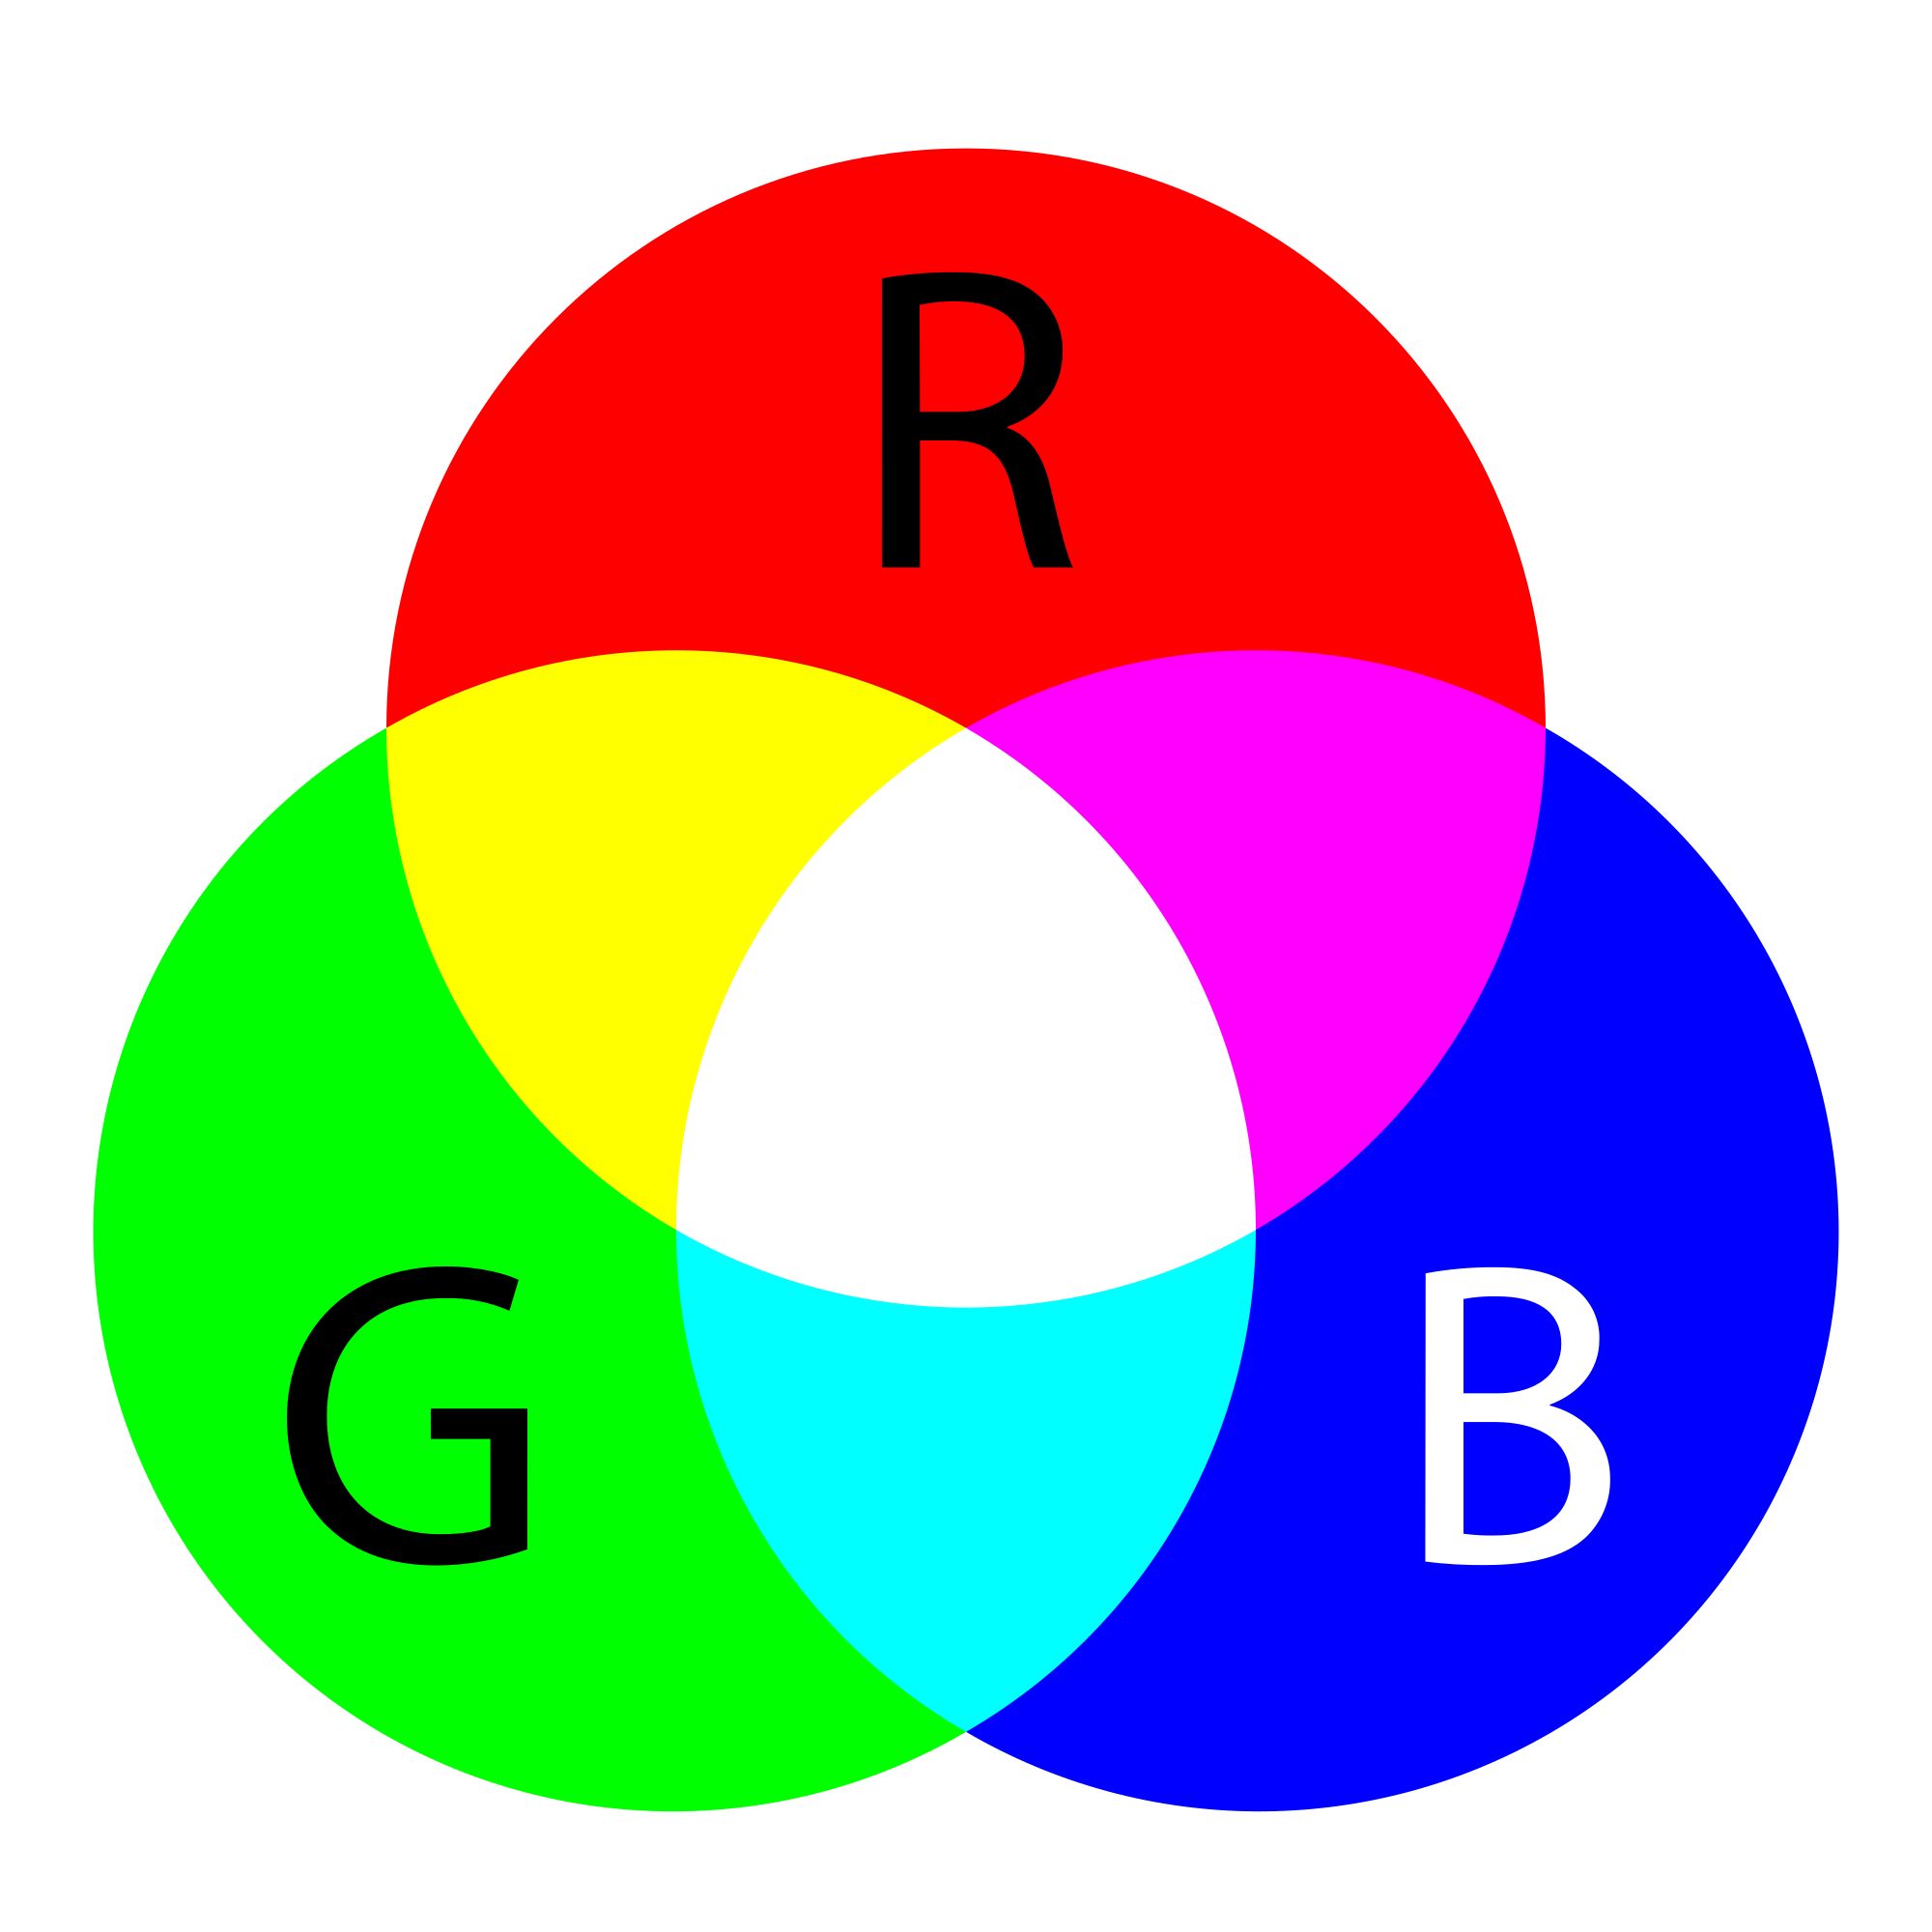
\includegraphics[width=0.3\linewidth]{resources/RGB}
    \end{center}
    \item Comment extraires des attributs du signal ?
  \end{itemize}
\end{frame}

\begin{frame}{Extraction d'attributs}{Méthodes pré-neuronales (1D signal)}
\begin{columns}
  \begin{column}{0.5\linewidth}
    \centering
    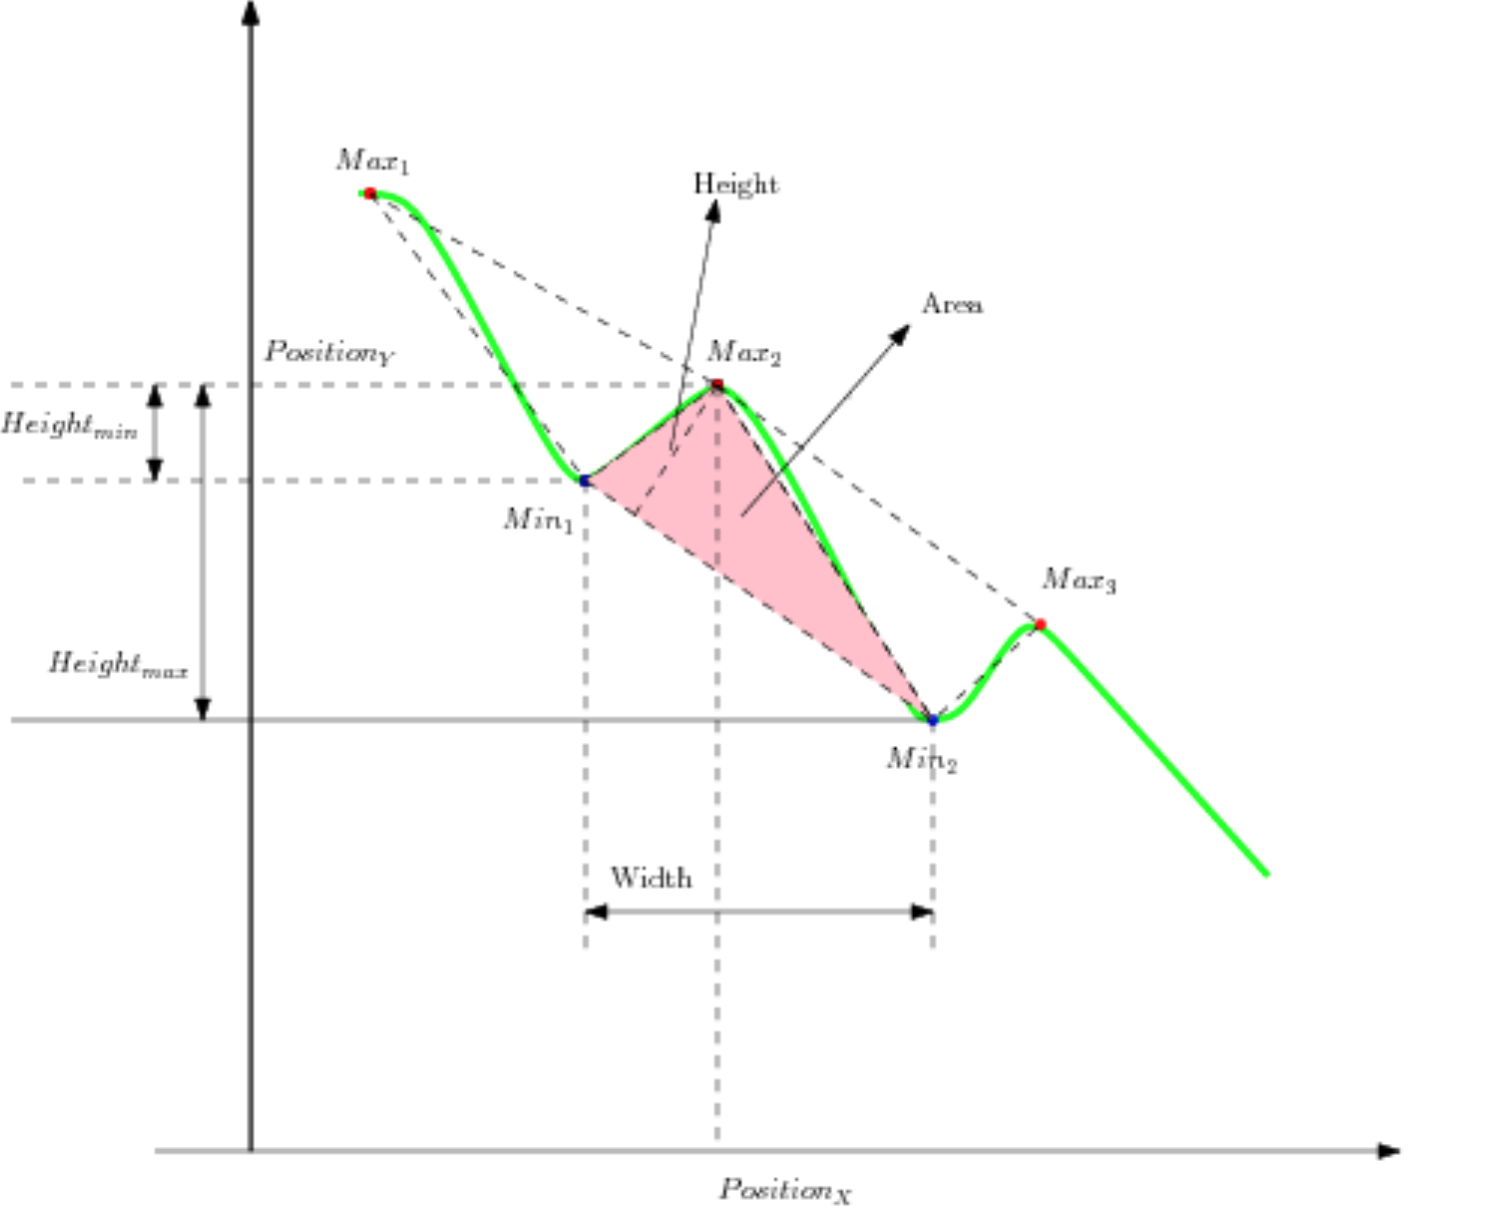
\includegraphics[width=0.9\linewidth]{resources/AA_exemple}
  \end{column}
  \begin{column}{0.5\linewidth}
    \centering
    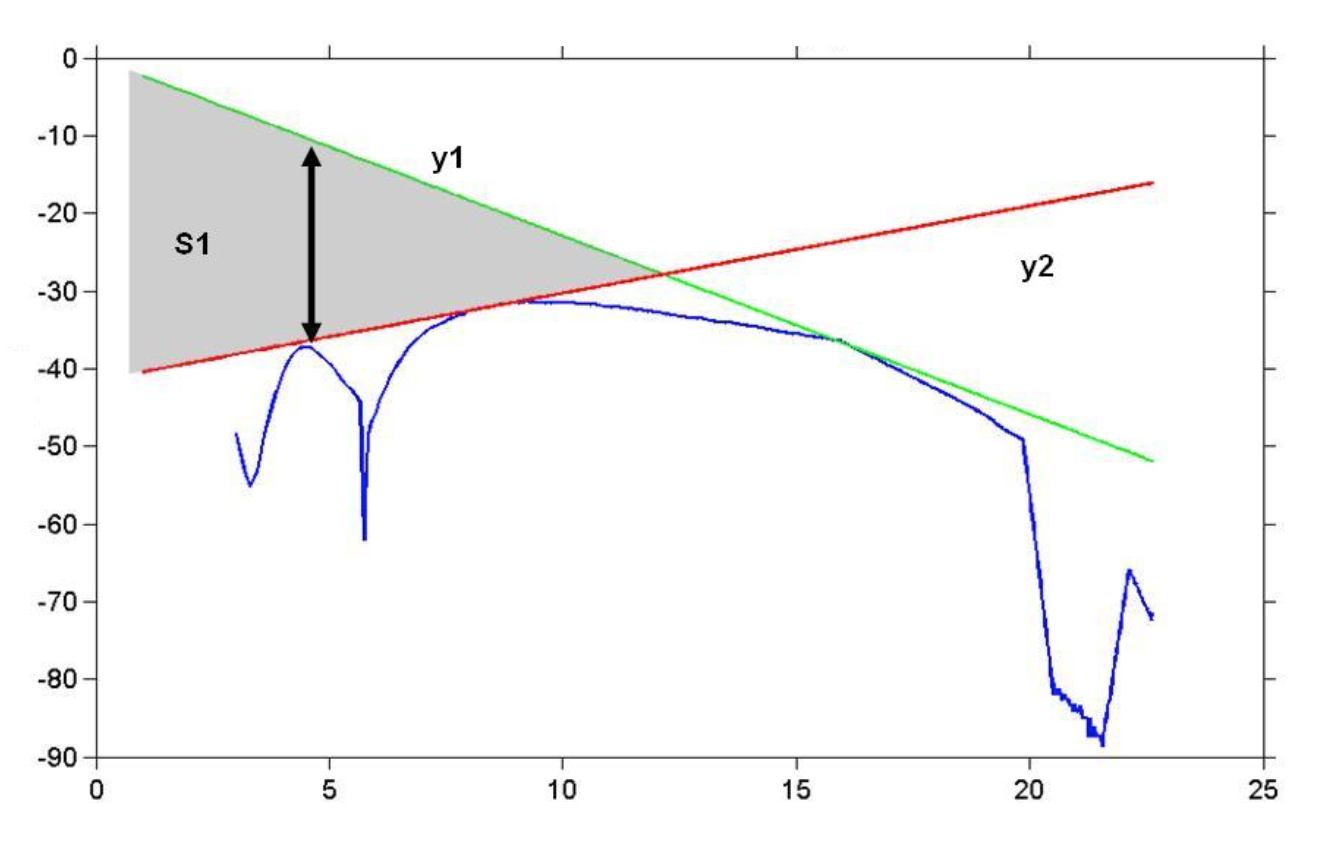
\includegraphics[width=0.9\linewidth]{resources/CC_example}
  \end{column}
\end{columns}
\end{frame}

\begin{frame}{Extraction d'attributs}{Méthodes pré-neuronales (2D signal)}
\centering
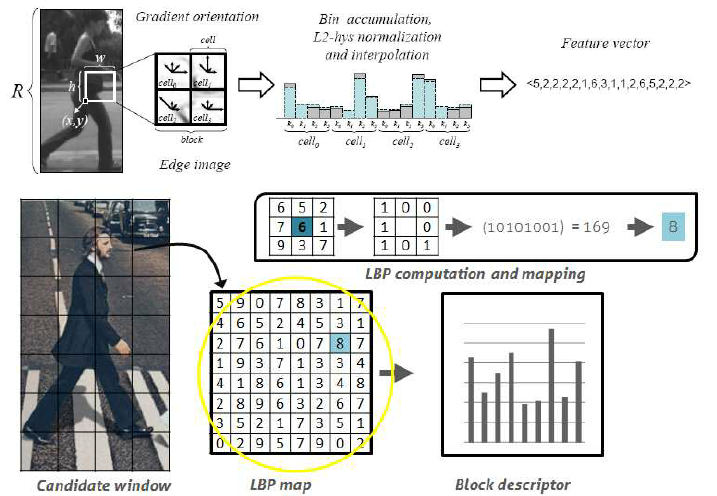
\includegraphics[width=0.9\linewidth]{resources/beatles}
\end{frame}

\begin{frame}{Convolutions}
	\centering
	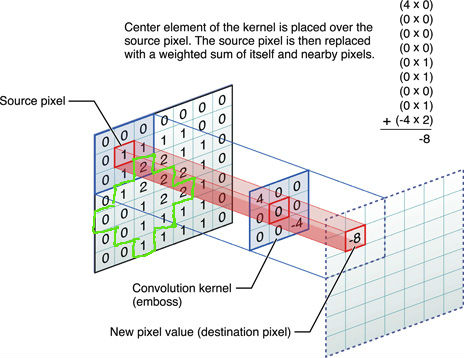
\includegraphics[width=0.9\linewidth]{resources/clem/convolution}
\end{frame}

\section{Réseaux de neurones}

\begin{frame}{Réseau de neurones profond}
  \begin{itemize}
  	\item 	Composé de plusieurs \textbf{\color{fibeamer@orange}couches}
  	\begin{itemize}
  		\item[$\rightarrow$] une couche \textbf{\color{fibeamer@orange}d'entrée} (attributs)
  		\item[$\rightarrow$] plusieurs couches \textbf{\color{fibeamer@orange} cachées} (calculs)
  		\item[$\rightarrow$] une couche de {\color{fibeamer@orange}sortie} (probabilités)
  	\end{itemize}
  \end{itemize}	
	\centering
	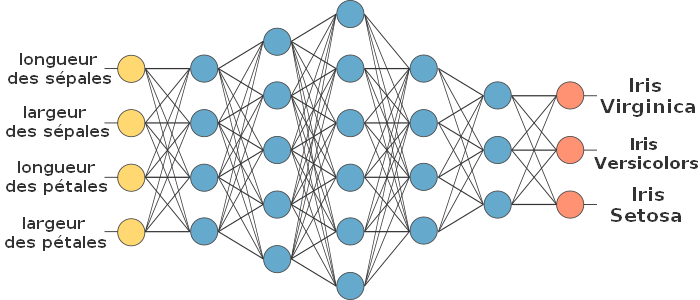
\includegraphics[width=1\linewidth]{resources/clem/simple_network2}
\end{frame}

\begin{frame}{Fonctionnement d'un neurone}
	\begin{itemize}
		\item Calcule une \textbf{\color{fibeamer@orange}somme} des entrées multipliées par des poids 
		\item Somme passée dans une \textbf{\color{fibeamer@orange}fonction d'activation}
	\end{itemize}	
	\centering
	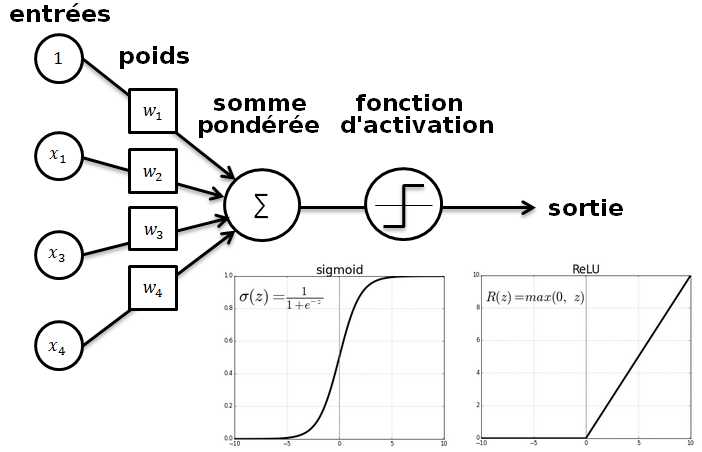
\includegraphics[width=0.9\linewidth]{resources/clem/perceptron2}
\end{frame}

\begin{frame}{Fonction d'erreur et backpropagation}
	\begin{itemize}
		\item Calcul de l'\textbf{\color{fibeamer@orange}erreur} 
		\begin{itemize}
		  \item[$\rightarrow$] différence entre la sortie et les valeurs attendues
		  \item[$\rightarrow$] plusieurs fonctions d'erreur possibles
		\end{itemize}
		\item Utilisation de l'erreur pour modifier les poids dans le réseau : backpropagation
	\end{itemize}	
	\centering
	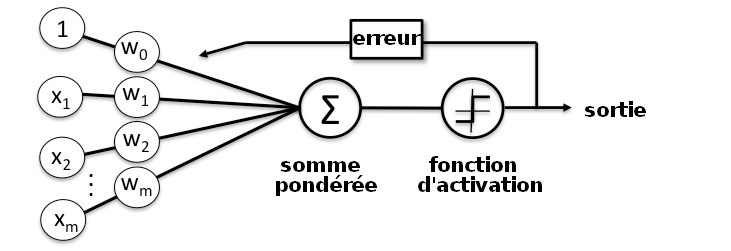
\includegraphics[width=1\linewidth]{resources/clem/error}
\end{frame}

\begin{frame}{Réseaux convolutionnels}
	\begin{itemize}
		\item Utilisés pour la reconnaissance d'image
		\begin{itemize}
			\item[$\rightarrow$] entrée : image
			\item[$\rightarrow$] couches de convolution
			\item[$\rightarrow$] couches de pooling
			\item[$\rightarrow$] couches denses
		\end{itemize}
		\item Le réseau apprend à reconnaitre des images et les labéliser
	\end{itemize}	
	\centering
	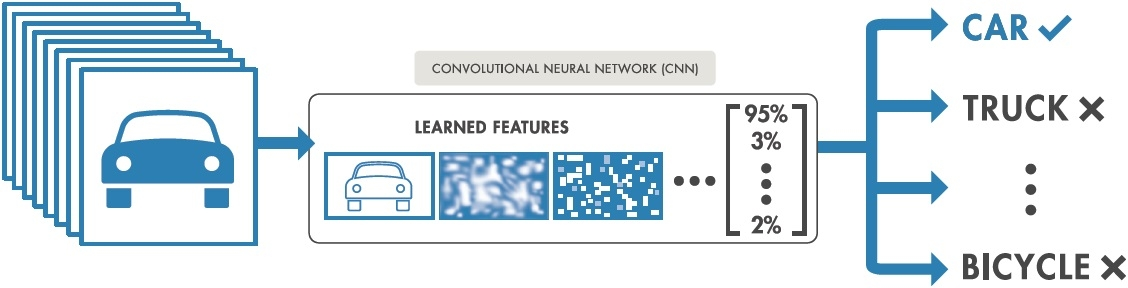
\includegraphics[width=1\linewidth]{resources/clem/car2}
\end{frame}

\begin{frame}{Réseaux convolutionnels}
	\begin{itemize}
		\item Utilisés pour la reconnaissance d'image
		\begin{itemize}
			\item[$\rightarrow$] entrée : image
			\item[$\rightarrow$] couches de convolution
			\item[$\rightarrow$] couches de pooling
			\item[$\rightarrow$] couches denses
		\end{itemize}
		\item Le réseau apprend à reconnaitre des images et les labéliser
	\end{itemize}	
	\centering
	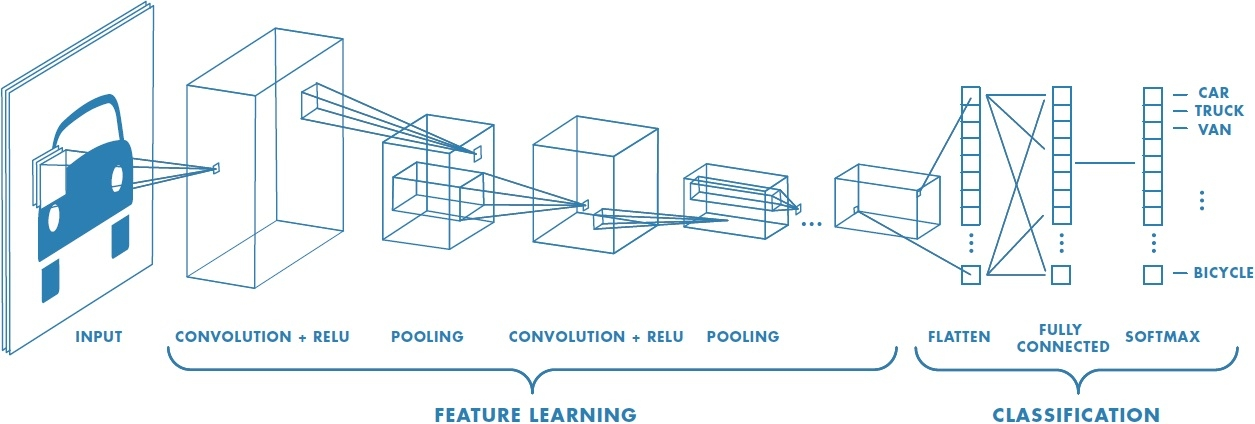
\includegraphics[width=1\linewidth]{resources/clem/convolutional_netowrk}
\end{frame}

\begin{frame}{Réseaux convolutionnels}	
	\centering
	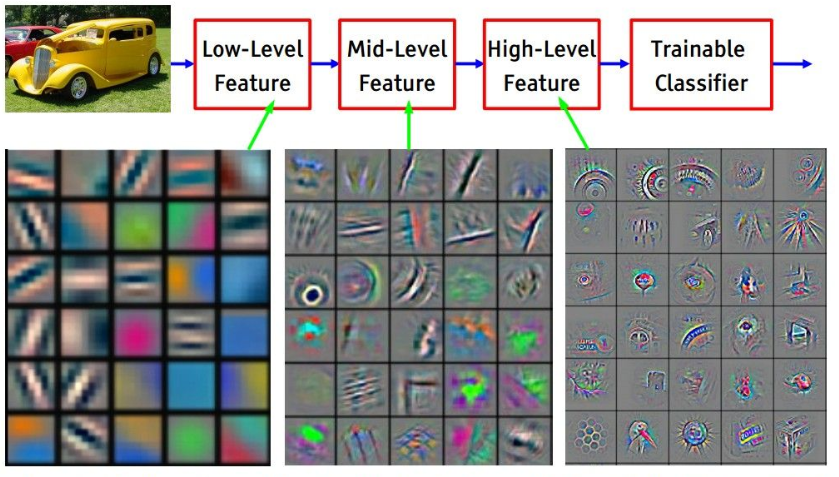
\includegraphics[width=1\linewidth]{resources/clem/features}
\end{frame}

\section{\'Etude de cas : âge et genre}
\subsection{Problème}
\begin{frame}{\'Etude de cas : âge et genre}
  \begin{itemize}
    \item
    \textbf{\color{fibeamer@orange}Projet} : créer un réseau de neuronnes convolutionnel
    permettant de détecter l'{\color{fibeamer@orange}âge} et le {\color{fibeamer@orange}genre} d'une personne sur une photographie.
    \item Projet réalisé avec python et le framework Keras (fournissant une API pour Tensorflow)
    \item \textbf{\color{fibeamer@orange}Base de données}: Wikipedia, openu (43390 images en tout)
    \item \textbf{\color{fibeamer@orange}\'Etapes :}
    \begin{enumerate}
      \item Régresseur de rotation
      \item Classifieur binaire homme/femme
      \item Régresseur d'âge
    \end{enumerate}
  \end{itemize}
\end{frame}
\subsection{Résistance aux rotations}

\begin{frame}{Résistance aux rotations}
  \textbf{\color{fibeamer@orange}Problématique :} le réseau doit reconnaître une personne en position \textit{penchée} et quelle que soit la rotation du visage.
  \begin{itemize}
    \item[$\rightarrow$] l'orientation du visage ne doit pas influencer le résultat !
  \end{itemize}
  \vspace{-.03\linewidth}
  \begin{figure}
    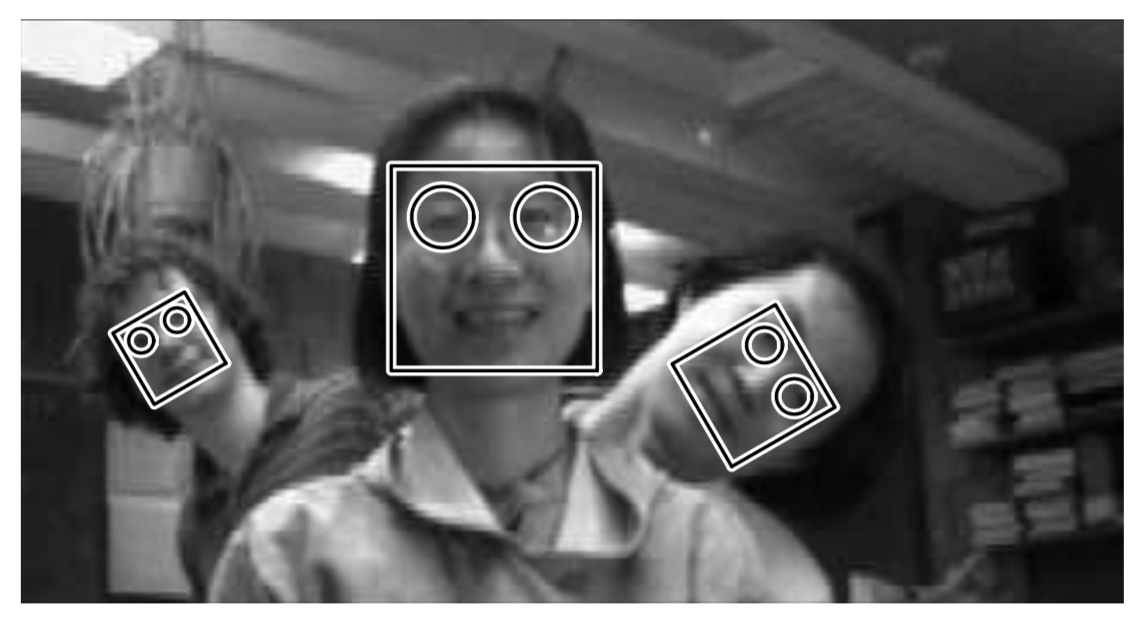
\includegraphics[width=0.8\linewidth]{resources/rotation2}
  \end{figure}
\end{frame}

\begin{frame}{Régresseur de rotation}
  \begin{itemize}
    \item On commence par créer un réseau de neuronnes convolutionnel jouant le rôle de \textbf{\color{fibeamer@orange}régresseur} de rotation
  \end{itemize}
  \begin{columns}
    \begin{column}{0.15\linewidth}\scriptsize
      \centering Entrée : image\\
      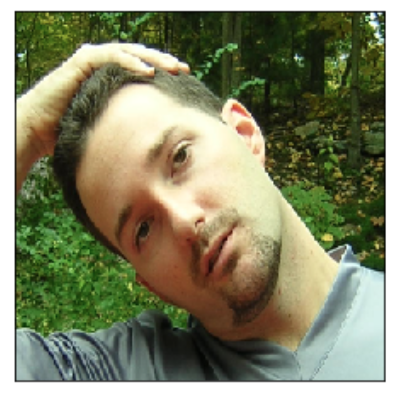
\includegraphics[width=\linewidth]{resources/rotation3} $\rightarrow$
    \end{column}
    \begin{column}{0.7\linewidth}
      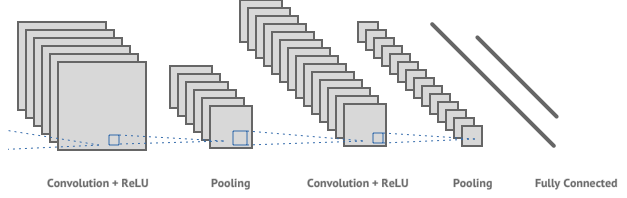
\includegraphics[width=\linewidth]{resources/convolutional_neural_network}
    \end{column}
    \begin{column}{0.15\linewidth}\scriptsize
      Sortie : angle\\
      $\rightarrow$ 45.94
    \end{column}
  \end{columns}
\end{frame}

\begin{frame}{Entraînement du régresseur de rotation}
  \begin{itemize}
    \item On utilise la base de données \textit{Openu}:
      toute les images de la base de données ont été pré-traitées au préalables et sont toutes parfaitement redressées
    \item On entraine le réseau en générant une rotation aléatoire pour chaque image, et chaque rotation correspond au label de cette image.
  \end{itemize}
  \begin{figure}
    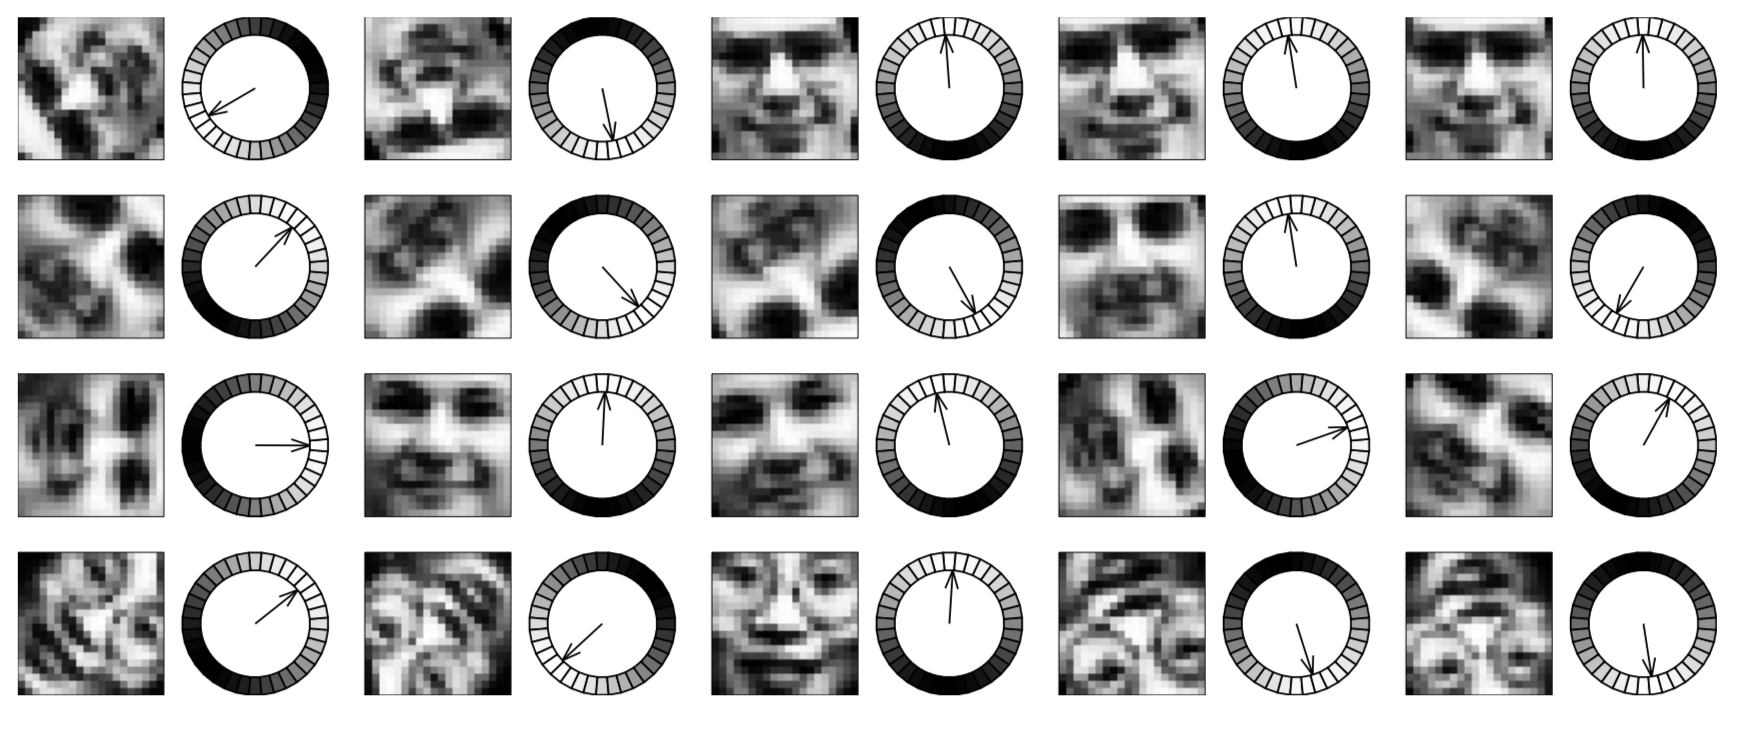
\includegraphics[width=0.6\linewidth]{resources/rotation}
  \end{figure}
\end{frame}

\begin{frame}{Régresseur de rotation}{Résultats}
  \begin{columns}
    \begin{column}{0.333\linewidth}\scriptsize
      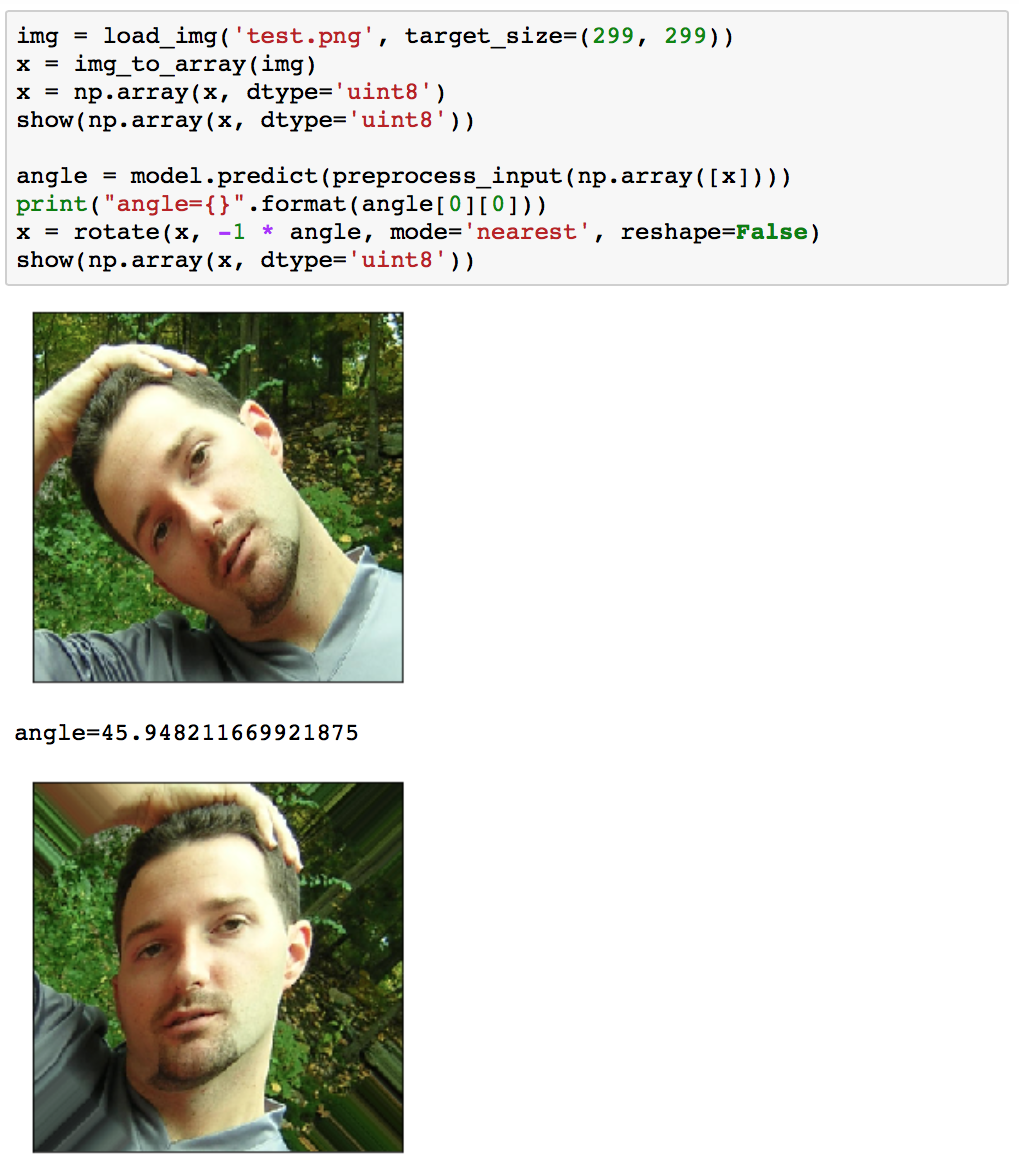
\includegraphics[width=\linewidth]{resources/rotationreg1}
    \end{column}
    \begin{column}{0.333\linewidth}
      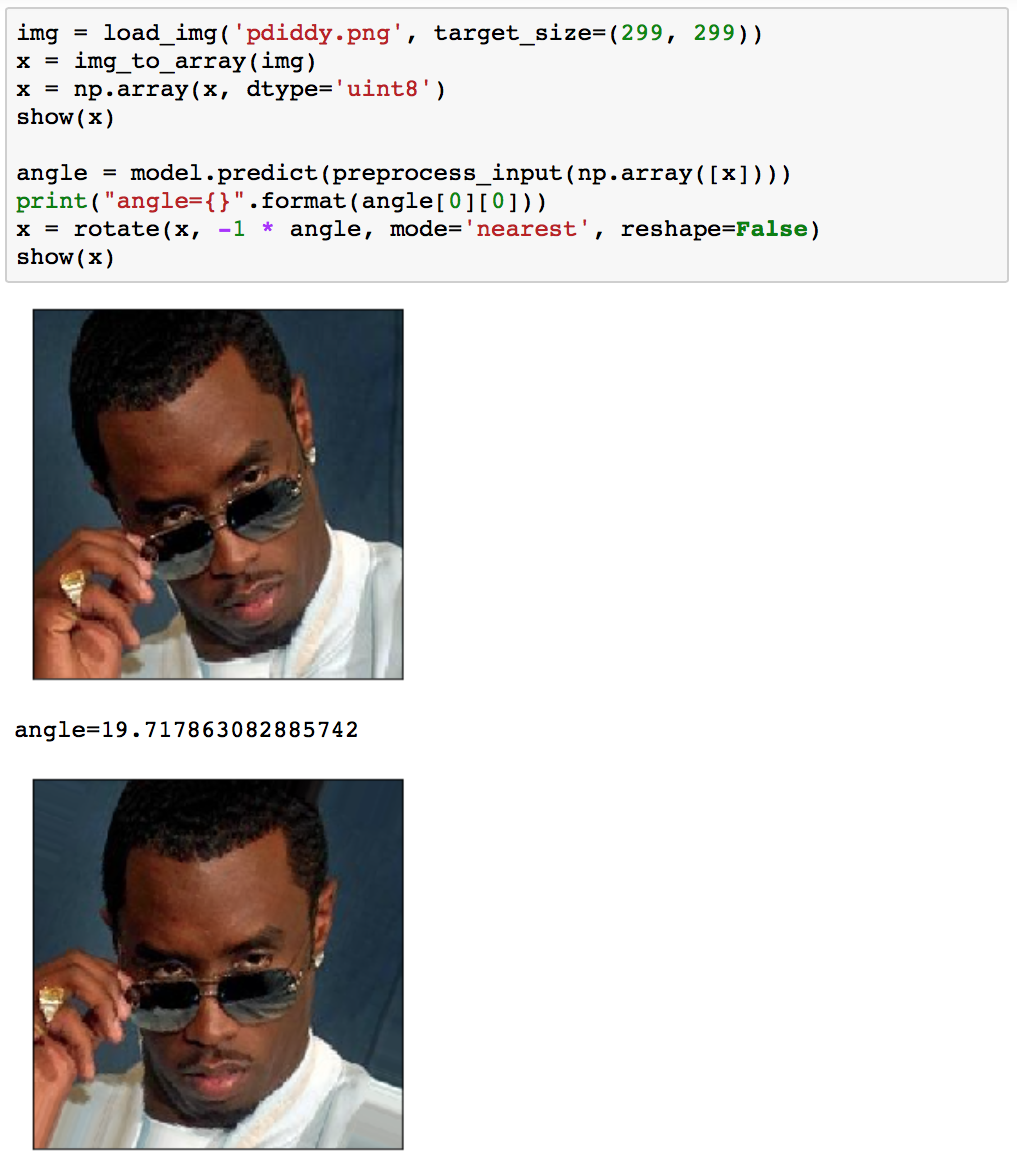
\includegraphics[width=\linewidth]{resources/rotationreg2}
    \end{column}
    \begin{column}{0.333\linewidth}\scriptsize
      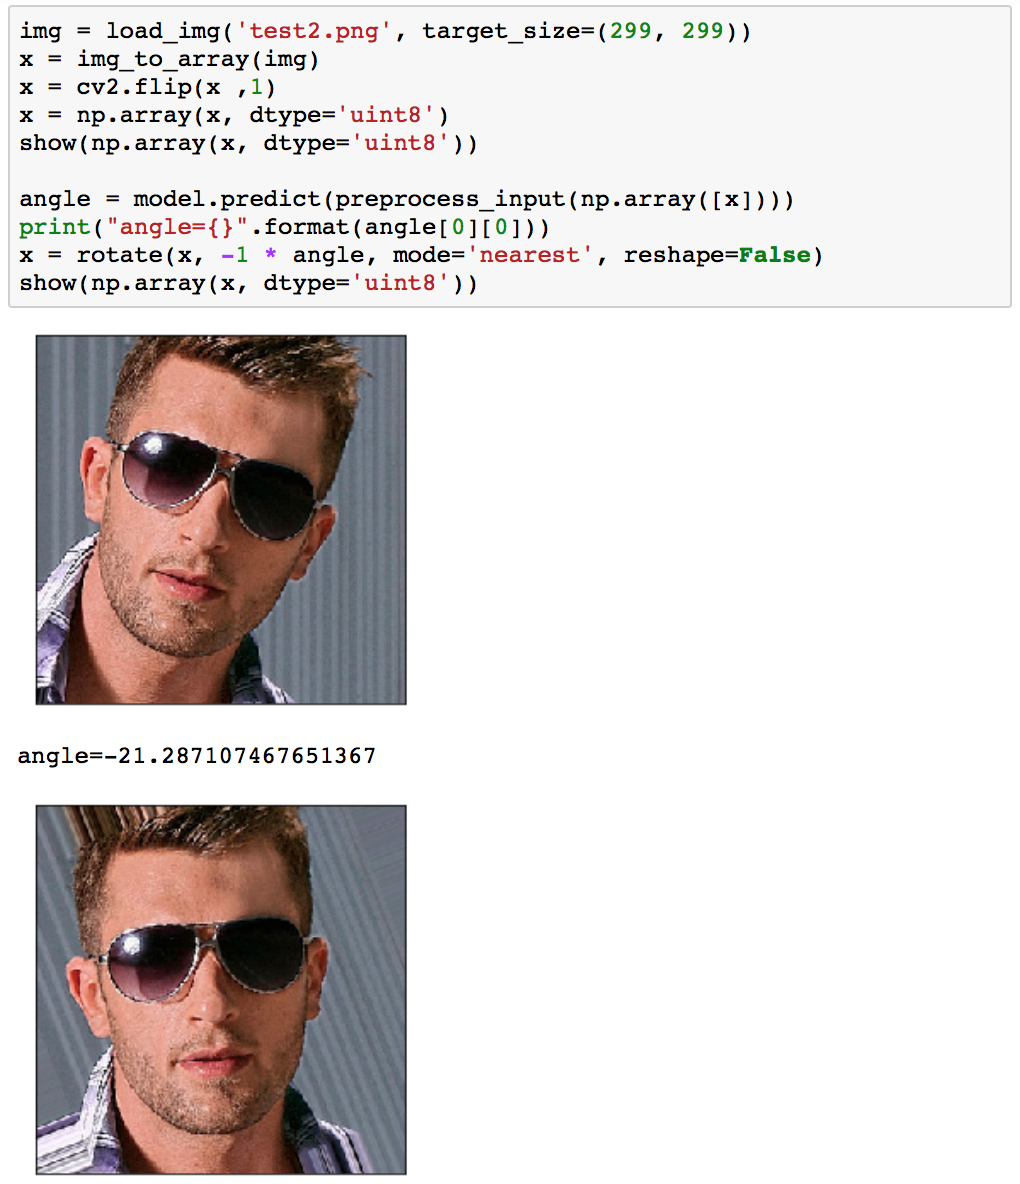
\includegraphics[width=\linewidth]{resources/rotationreg3}
    \end{column}
  \end{columns}

\end{frame}

\begin{frame}{Classifieur homme/femme}
  \begin{itemize}
    \item Basé sur le réseau \textbf{Xception} de Google
    \begin{itemize}
      \item profondeur : 126
      \item paramètres : 22,910,480
      \item originalement entrainé pour reconnaitre les images de la base de données \textbf{image net} (pas de lien avec notre problème)
    \end{itemize}
    \begin{figure}
      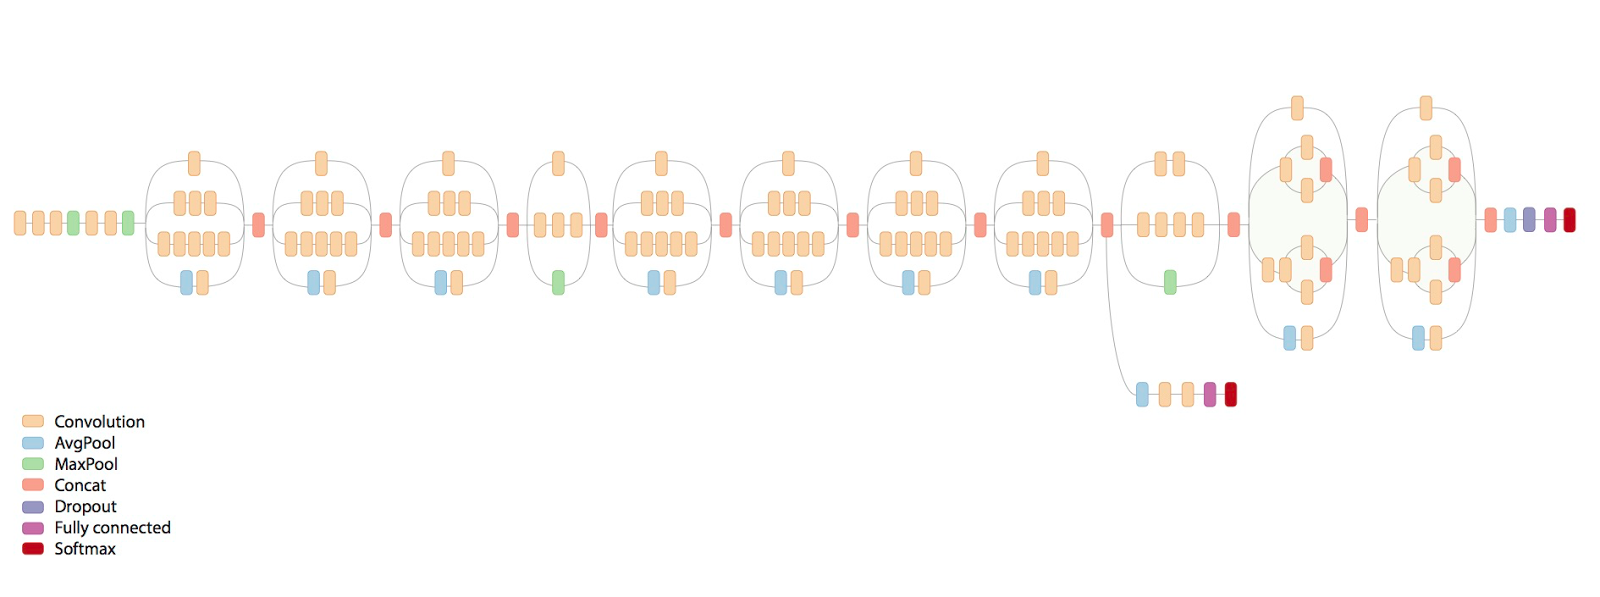
\includegraphics[width=\linewidth]{resources/Xception}
    \end{figure}
  \end{itemize}
\end{frame}

\subsection{Classification de genre}

\begin{frame}{Classifieur homme/femme}{Apprentissage}\footnotesize
  \vspace{-.06\linewidth}
    \begin{figure}
      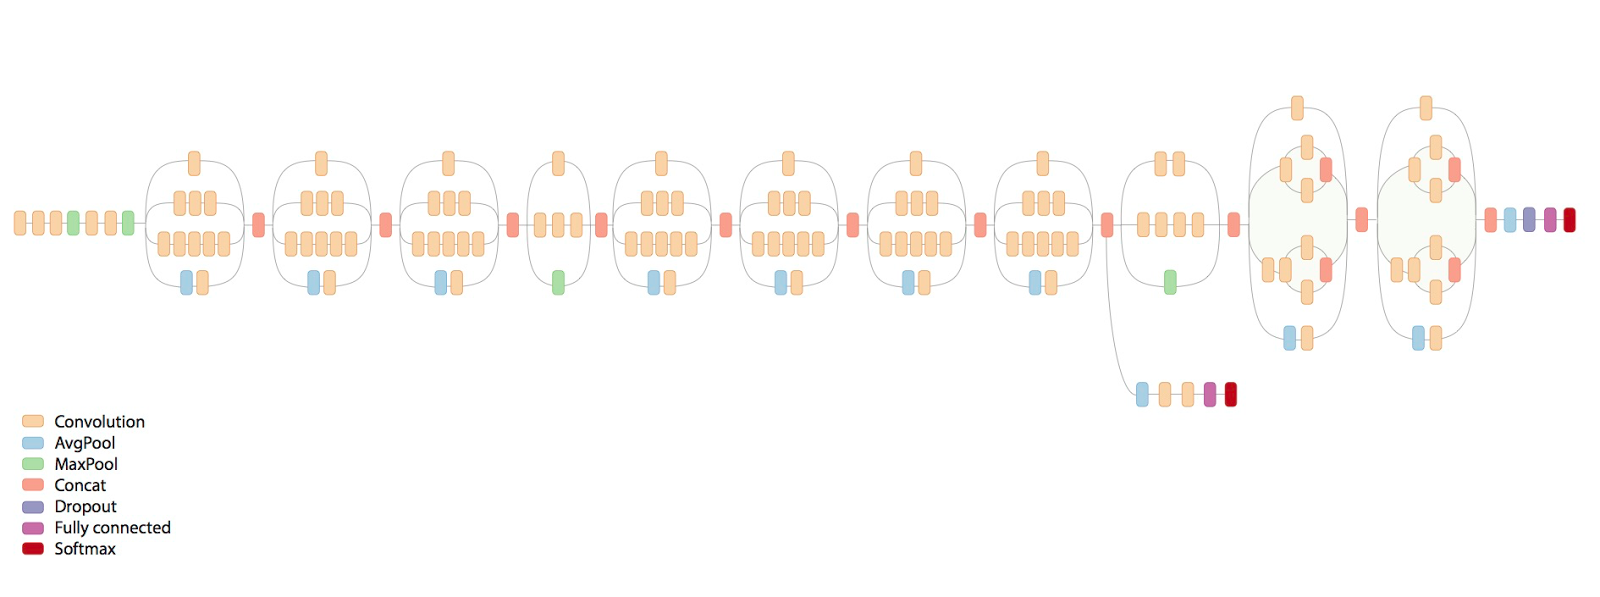
\includegraphics[width=\linewidth]{resources/Xception}
    \end{figure}
  \vspace{-.05\linewidth}
\begin{itemize}
    \item Apprentissage par \textbf{\color{fibeamer@orange}transfert}: on utilise le réseau Xception de Google déjà entrainé en ``gelant''
    les 115 premières couches et en entrainant uniquement les couches restantes (top layers) pour notre problème.
    \item \textbf{\color{fibeamer@orange}Affinement du résultat} : on répète l'opération en gelant cette fois la moitié du réseau, mais avec un taux d'apprentissage plus faible
\end{itemize}
\end{frame}

\begin{frame}{Classifieur homme/femme}{Apprentissage}
\begin{itemize}
  \item Le réseau doit être le plus \textbf{\color{fibeamer@orange}robuste} possible face aux translations, aux zooms, etc.
  \begin{itemize}
    \item[$\rightarrow$] Le sexe d'une personne ne doit pas changer en fonction de la position de son visage sur l'image
  \end{itemize}
  \item Entraînement par \textbf{\color{fibeamer@orange}augmentation de données}
\end{itemize}
  \vspace{-0.03\linewidth}
  \begin{figure}
    \centering
    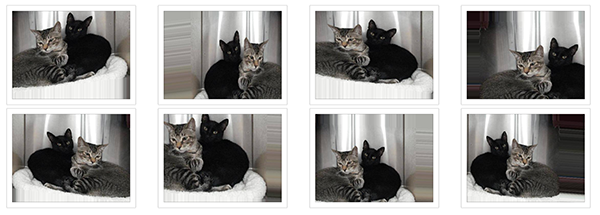
\includegraphics[width=0.8\linewidth]{resources/data-augmentation.png}
  \end{figure}
\end{frame}

\begin{frame}{Classifieur homme/femme}{Résultats}
    \begin{figure}
      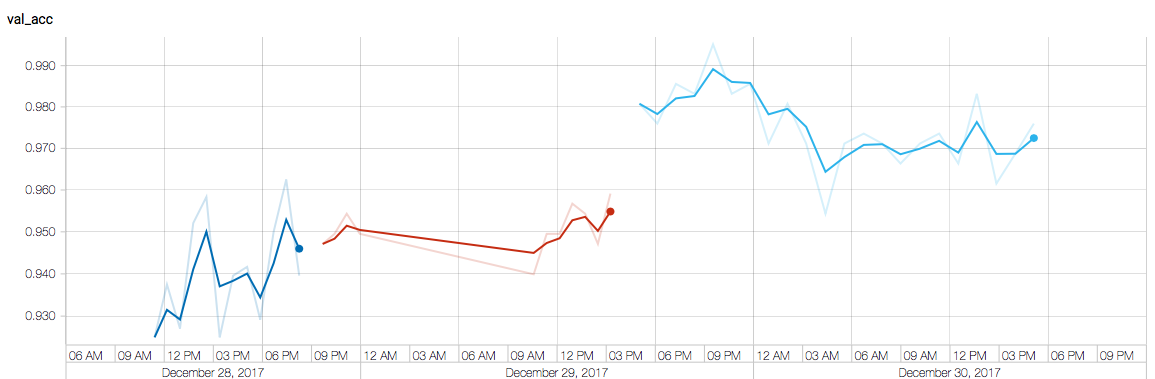
\includegraphics[width=\linewidth]{resources/fine-tuning}
      \caption{Entraînement du modèle - en bleu clair : phase d'affinement}
    \end{figure}
\begin{itemize}
  \item Accuracy : $99.52 \%$ (bornée) sur l'ensemble de test
\end{itemize}
\end{frame}

\subsection{Régresseur d'âge}

\begin{frame}{Régresseur d'âge}
  \begin{itemize}
    \item Apprentissage par transfert (depuis Xception)
    \item Entraînement par augmentation de données
    \item Les 20 dernières couches de convolution sont modifiées
    \begin{itemize}
      \item[$\rightarrow$] les dernières couches de convolution {\color{fibeamer@orange}se divisent en $2$ en fonction du sexe prédit par le réseau classifieur de genre}
    \end{itemize}
  \end{itemize}
    \begin{figure}
      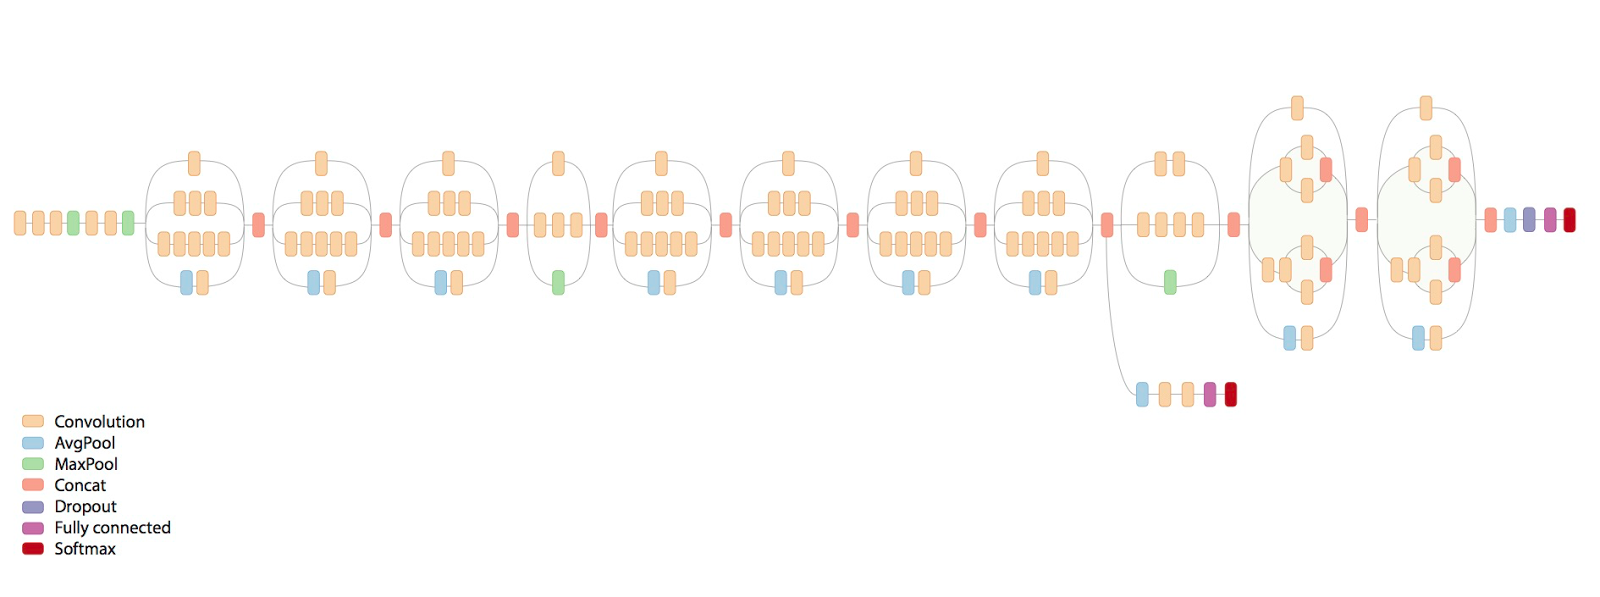
\includegraphics[width=\linewidth]{resources/Xception}
    \end{figure}
\end{frame}

\begin{frame}{Régresseur d'âge}
  \vspace{-.11\linewidth}
  \begin{figure}
    \centering\hspace{.1\linewidth}
    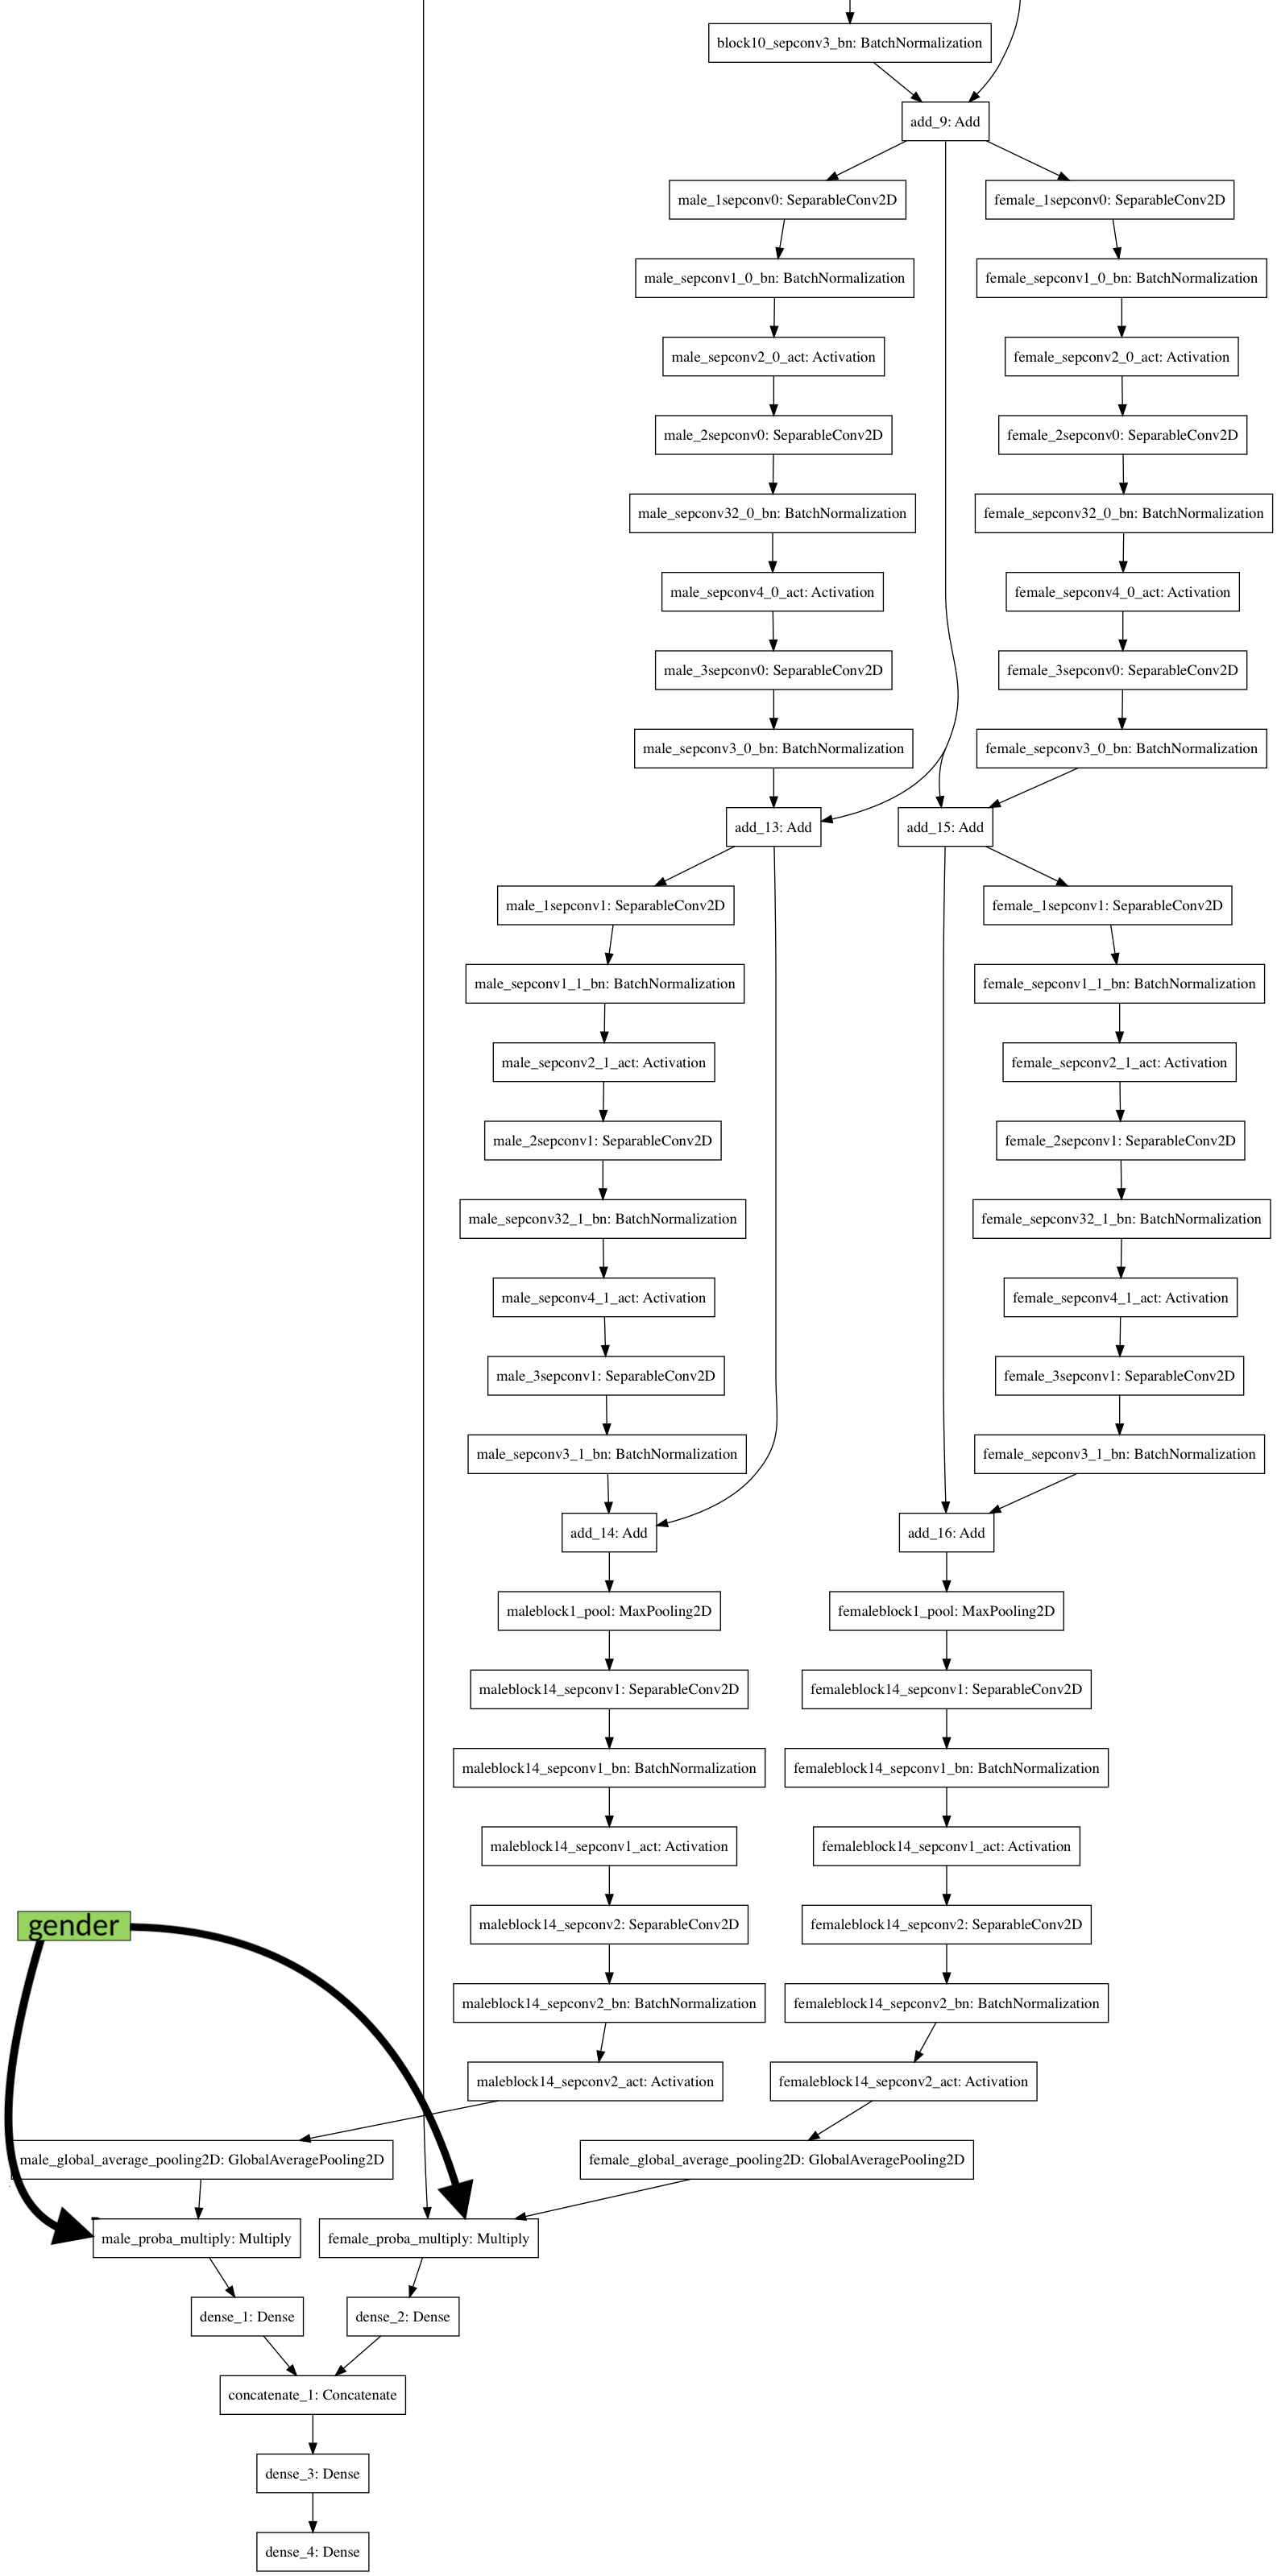
\includegraphics[width=0.4\linewidth]{resources/age_regressor}
  \end{figure}
\end{frame}


\begin{frame}{Régresseur d'âge}{Résultats}
    \begin{figure}
      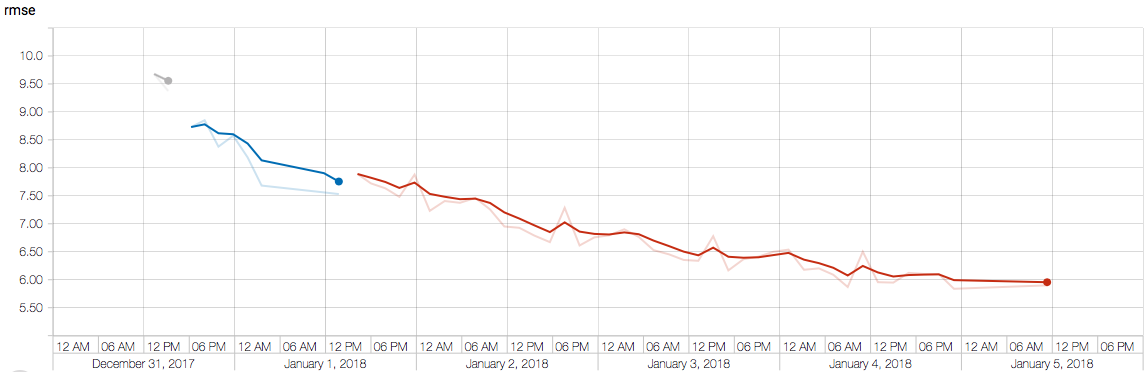
\includegraphics[width=\linewidth]{resources/age-reg}
      \caption{Entraînement du modèle}
    \end{figure}
    \vspace{-.05\linewidth}
\begin{itemize}
  \item rmse (root mean square error) : $5.88$
  \begin{itemize}
    \item[$\rightarrow$] l'âge d'une personne est dans une intervale $\pm 5.88$ de la prédiction
  \end{itemize}
    \item Entraînement limité par le hardware
\end{itemize}
\end{frame}

\subsection{Résultats}

\begin{frame}{Résultats}
  \begin{columns}
    \begin{column}{0.6\linewidth}
      \inputminted[fontsize=\scriptsize]{python}{code2.py}
    \end{column}
    \begin{column}{0.4\linewidth}
      \centering
      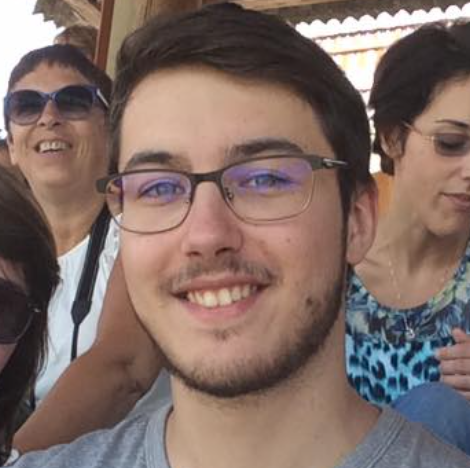
\includegraphics[width=\linewidth]{resources/clem}
    \end{column}
  \end{columns}
    $\rightarrow$ age : [[ 24.6701107]]
\end{frame}

\begin{frame}{Résultats}
  \begin{columns}
    \begin{column}{0.6\linewidth}
      \inputminted[fontsize=\scriptsize]{python}{code1.py}
    \end{column}
    \begin{column}{0.4\linewidth}
      \centering
      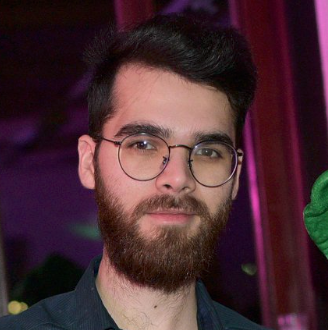
\includegraphics[width=\linewidth]{resources/Flo}
    \end{column}
  \end{columns}
    $\rightarrow$ age : [[25.11619949]]
\end{frame}

\begin{frame}{Résultats}
  \begin{columns}
    \begin{column}{0.6\linewidth}
      \inputminted[fontsize=\scriptsize]{python}{code3.py}
    \end{column}
    \begin{column}{0.4\linewidth}
      \centering
      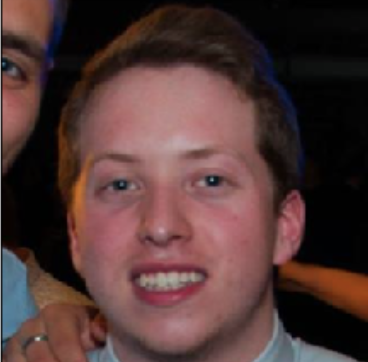
\includegraphics[width=\linewidth]{resources/jerem}
    \end{column}
  \end{columns}
    $\rightarrow$ age : [[24.46559525]]
\end{frame}

\begin{frame}{Résultats}
  \begin{columns}
    \begin{column}{0.6\linewidth}
      \inputminted[fontsize=\scriptsize]{python}{code4.py}
    \end{column}
    \begin{column}{0.4\linewidth}
      \centering
      
\includegraphics[width=\linewidth]{resources/giorgio-armani}
    \end{column}
  \end{columns}
    $\rightarrow$ age : [[29.9426403]]
\end{frame}

\begin{frame}{Résultats}
  \begin{columns}
    \begin{column}{0.6\linewidth}
      \inputminted[fontsize=\scriptsize]{python}{code5.py}
    \end{column}
    \begin{column}{0.4\linewidth}
      \centering
      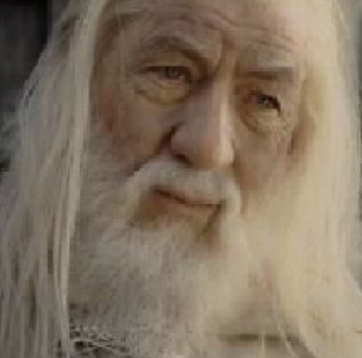
\includegraphics[width=\linewidth]{resources/gandalf}
    \end{column}
  \end{columns}
    $\rightarrow$ age : [[90.07471466]]\\
    Résultat réaliste
\end{frame}

\begin{frame}{Résultats}
  \begin{columns}
    \begin{column}{0.6\linewidth}
      \inputminted[fontsize=\scriptsize]{python}{code6.py}
    \end{column}
    \begin{column}{0.4\linewidth}
      \centering
      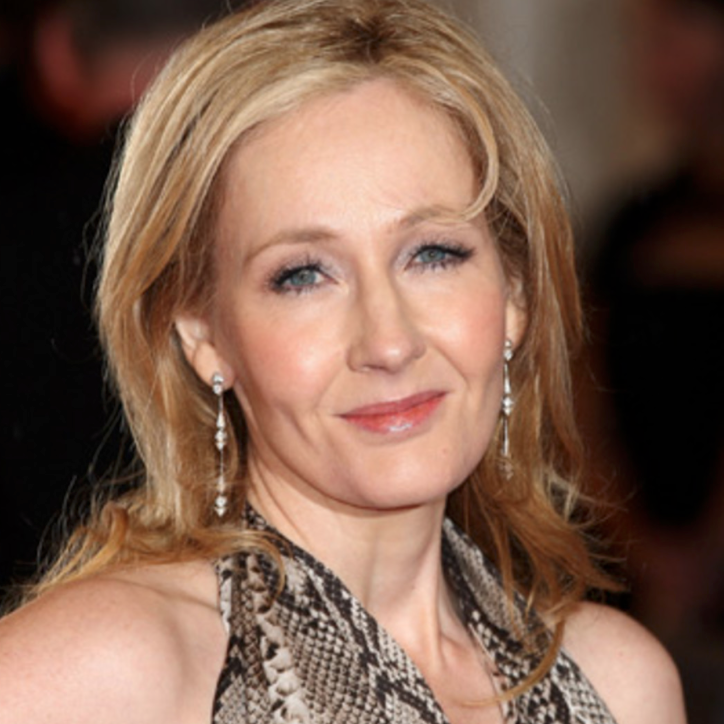
\includegraphics[width=\linewidth]{resources/JKrowling}
    \end{column}
  \end{columns}
    $\rightarrow$ age : [[52.0241394]]\\
    Âge réel : 52 ans !
\end{frame}

\subsection{}
% \begin{frame}[allowframebreaks]
%         \nocite{*}
%         \frametitle{Références}
%       \printbibliography
% \end{frame}

\section{Conclusion}

\begin{frame}{Applications}
	Le machine learning, et particulièrement le deep learning 
	\begin{itemize}
		\item est utilisé dans l'industrie
		\item a de vagues applications
		\item permet la découverte de données
	\end{itemize}
	
	Nous présentons ci-après plusieurs applications concrètes
\end{frame}

\begin{frame}
	\frametitle{Speech recognition}
	
	\begin{figure}
		\centering
		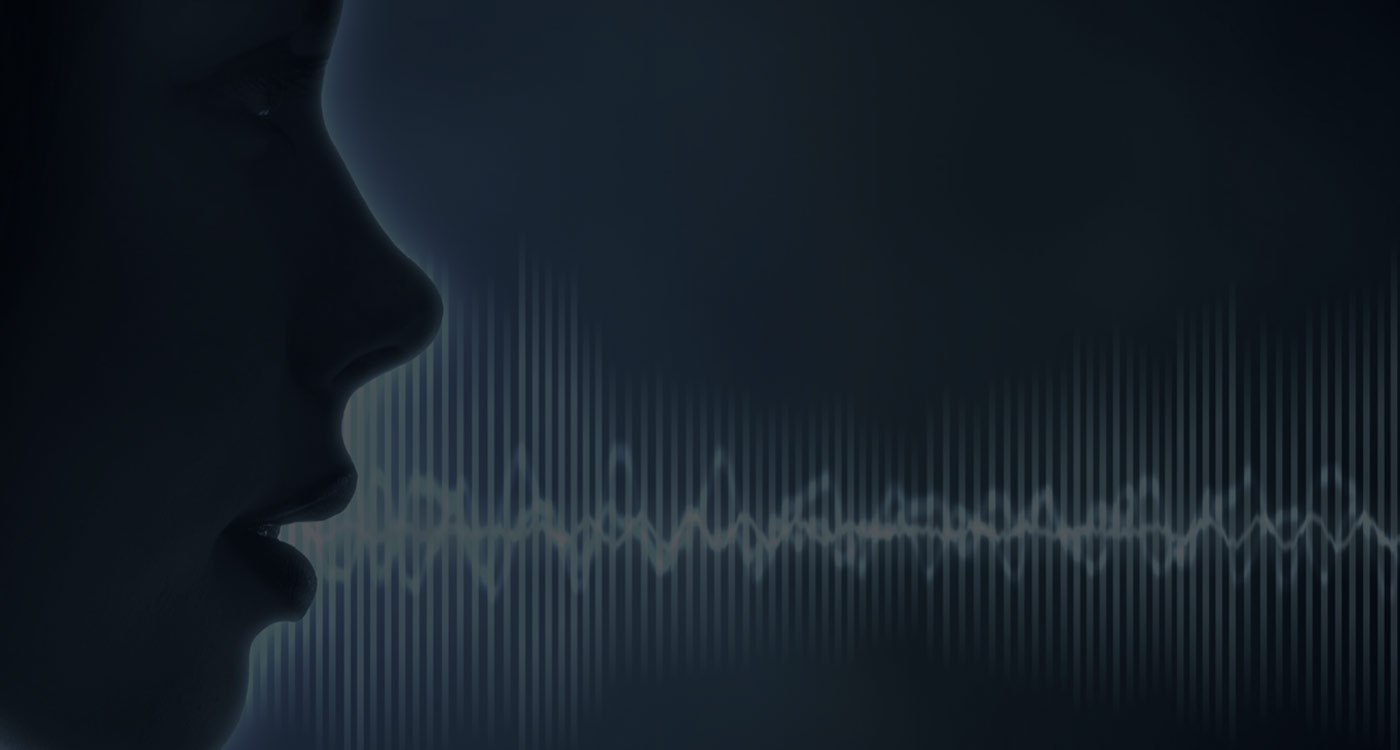
\includegraphics[width=1\linewidth]{resources/speech}
	\end{figure}
	
\end{frame}

\begin{frame}
	\frametitle{Vérification de la qualité}
	
	\begin{figure}
		\centering
		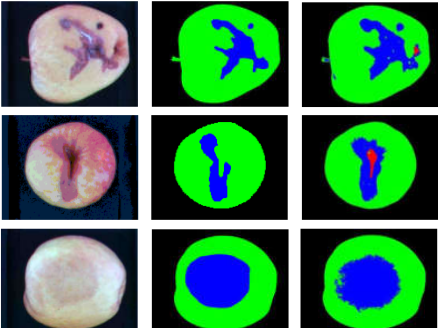
\includegraphics[width=0.8\linewidth]{resources/quality}
	\end{figure}
	
\end{frame}


\begin{frame}
	\frametitle{Maintenance prédictive}
	
	\begin{figure}
		\centering
		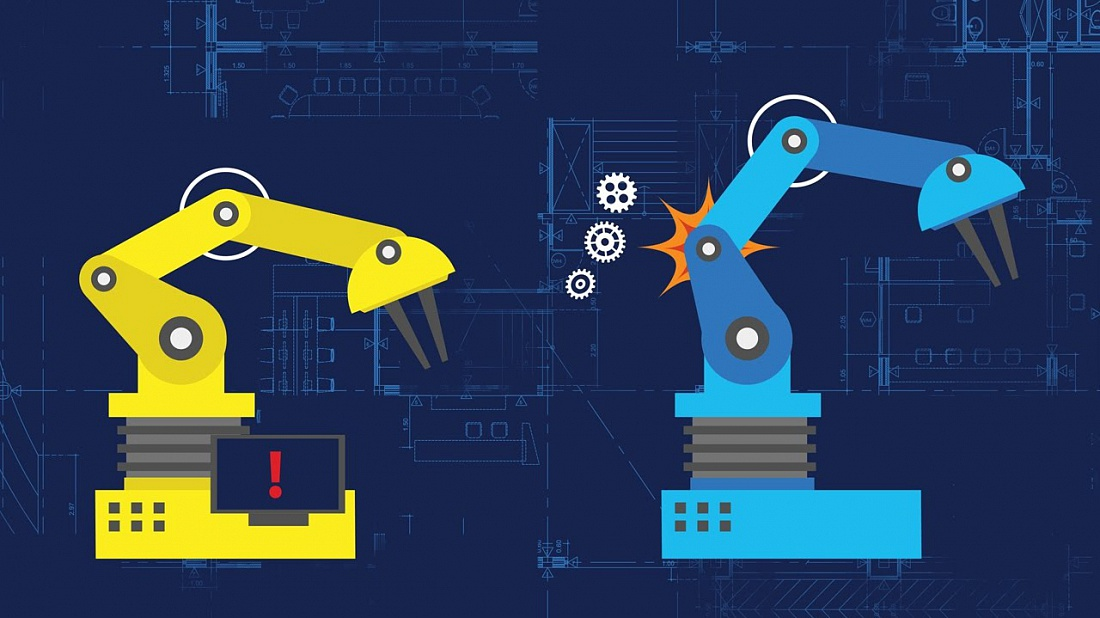
\includegraphics[width=1\linewidth]{resources/maintenance}
		
	\end{figure}
	
\end{frame}

\begin{frame}
	\frametitle{Médecine}
	
	\begin{figure}
		\centering
		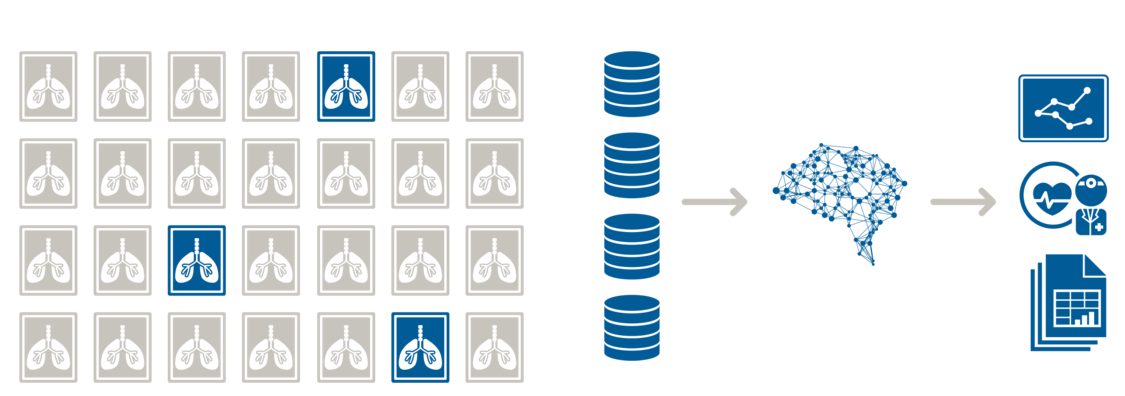
\includegraphics[width=1\linewidth]{resources/medical}
	\end{figure}
	
\end{frame}

\begin{frame}
	\frametitle{Finance}
	
	\begin{figure}
		\centering
		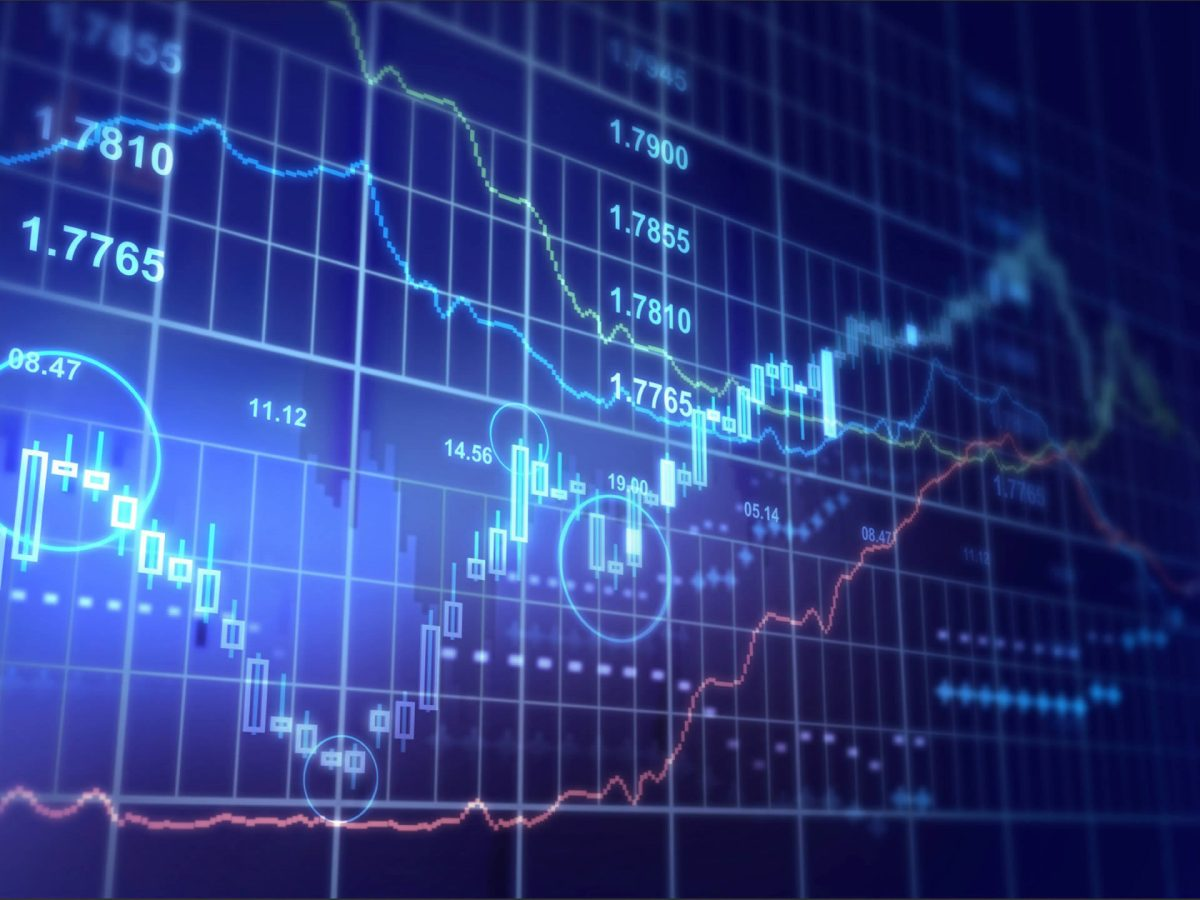
\includegraphics[width=0.9\linewidth]{resources/stock}
		
	\end{figure}
	
	
\end{frame}

\begin{frame}
	\frametitle{Reconnaissance de texte}
	
	\begin{figure}
		\centering
		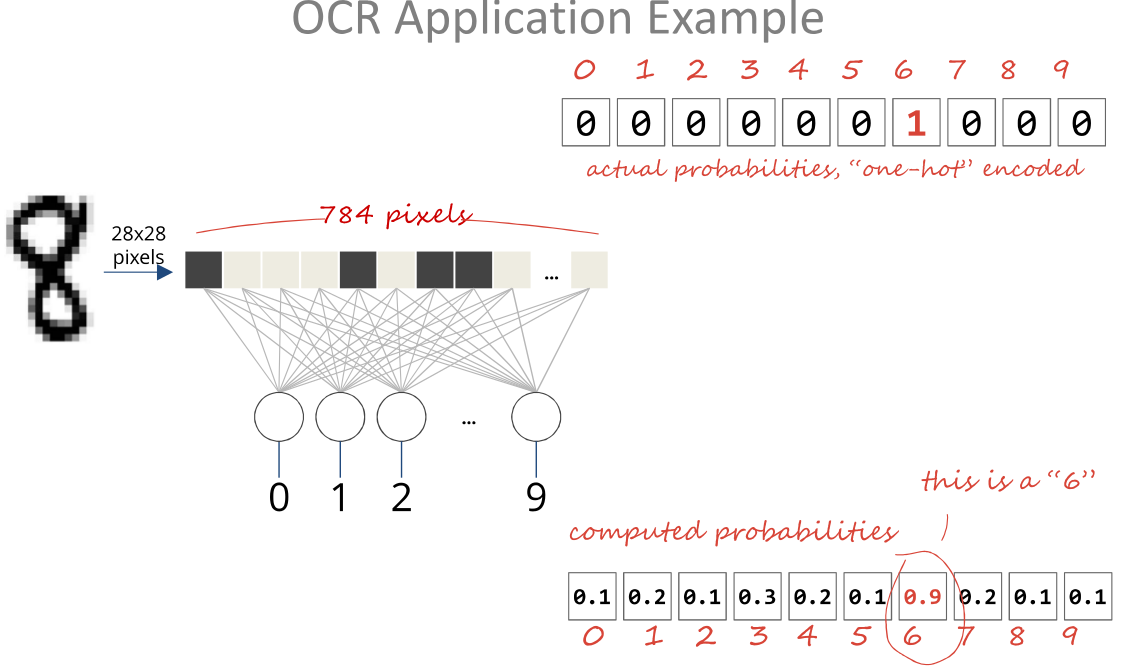
\includegraphics[width=1\linewidth]{resources/text}
	\end{figure}
	
\end{frame}

\begin{frame}
	\frametitle{Inconvénients}
	
	mark zuckerberg slide
		\begin{figure}
			\centering
			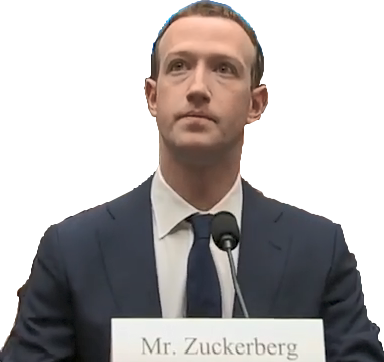
\includegraphics[width=0.72\linewidth]{resources/clem/zucc}
		\end{figure}
\end{frame}
\end{document}
